\documentclass[12pt]{extarticle}
%\documentclass{article}
\usepackage[utf8]{inputenc}

\usepackage{graphicx}
\usepackage{framed}
\usepackage[normalem]{ulem}
\usepackage{amsmath}
\usepackage{amsthm}
\usepackage{amssymb}
\usepackage{amsfonts}
\usepackage{enumerate}
\usepackage{hyperref} 
\usepackage{subfig}
\usepackage{pdflscape}
\usepackage{rotating}

\usepackage[top=1 in,bottom=1in, left=1 in, right=1 in]{geometry}
%\usepackage{fullpage} % Package to use full page
\usepackage{parskip} % Package to tweak paragraph skipping
\usepackage{enumitem}
\usepackage{datetime}
\usepackage{ragged2e}
\usepackage{subcaption}
\usepackage{multicol}
\usepackage{fancyvrb}
\usepackage{relsize}
\usepackage{caption}
\usepackage{float}
\restylefloat{table}
\usepackage[table,xcdraw]{xcolor}
\usepackage{longtable}
\usepackage[official]{eurosym}
\usepackage{mdframed}
\usepackage{multirow}

%\title{OD Final Project}
%\author{amaliavradi }
%\date{June 2019}

%opening



\begin{document}


{\fontfamily{cmr}\selectfont
\title{ \normalsize \textsc{}
		\\ [2.0cm]
		\LARGE \textbf{{Exploratory Multivariate Analysis on World Happiness Report}\\
		\vspace*{2\baselineskip}
		\normalsize \today\\
		\\
		\normalsize BarcelonaTech UPC\\
		\normalsize MIRI Data Science - MVA\\
		\vspace*{15\baselineskip}
		}
}

\date{}

\author{\
\texttt{Ricard Monge Calvo}\\
ricard.monge.calvo@est.fib.upc.edu
\and
\texttt{Javier Flores }\\
javier.de.jesus.flores@est.fib.upc.edu
\and
\texttt{Amalia Alkisti Vradi}\\
amalia.vradi@est.fib.upc.edu
\and
}

}

\maketitle
\thispagestyle{empty}
\newpage

\tableofcontents

\newpage

\section{Introduction}
Happiness is widely considered as the most important part in life, we can define happiness as the joy that we feel when we are striving after our potential.  There are many research studies focusing on which factors have influence over happiness and different ways to measure it more accurately. Thanks to the effort made in these studies we have systematic and widely accepted happiness measurements. Organizations like the United Nations (UN) have invited countries to measure the collective happiness of their population through the World Happiness Report  (WHR) and use this data as a guide to improve their societies.

The effort of the United Nation’s to define a happiness score is within the goal of defining and setting a holistic definition of development. The main driver for this initiative is to help the governments and the global and local authorities to define public policies towards a new economic paradigm, based on happiness and well-being. To this end, the World Happiness Report is being published every year, providing as well the data to the public.

In this report, a multivariate analysis is made from the World Happiness Report of 2019. The purpose of our analysis is to reveal the hidden information regarding happiness contained in the data that have been gathered. We conducted a multivariate exploration and performed visualizations and clustering of our data with the corresponding interpretation of our results in order to explore our available data. We wonder about topics such as what are the factors that contribute the most in a society for the people to feel happy. What’s more, we discuss if there are any patterns among the countries that score the similar happiness scores.

To conclude, we use our obtained knowledge in order to build a model to predict the happiness score of a country for the next year, and compare our predictions with the real scores delivered in the WHR 2019.



\newpage
\section{Data}

The World Happiness Report is a yearly publication, with the first report being published in 2012. Along with every edition, the organization publishes the corresponding data in their website\footnote{https://worldhappiness.report/}. The data is collected from people from around the world, in over 150 countries, and are based on poll questions. The questions focus on six different aspects of society and life, in order to measure how these contribute to making life evaluations higher. Those aspects are economic production, social support, life expectancy, freedom, generosity, and absence of corruption.

In particular, the dataset for WHR 2019 originally contained 27 variables on which we performed a detailed pre-processing, which we comment in detail in the next section. In the following table, we provide a short summary of some of the most important variables considered:


\begin{longtable}[c]{cl}
    \rowcolor[HTML]{C0C0C0} 
    \textbf{Variable} & \multicolumn{1}{c}{\cellcolor[HTML]{C0C0C0}\textbf{Variable Definition}} \\\hline \endhead
             Happiness Score & National average response to the question of life evaluations. \\\hline
             Log GDPpc & Logarithm of GDP per capita, in purchasing power parity. \\\hline
             Social Support & \begin{tabular}{@{}l@{}}Average of binary response to the question of whether \end{tabular} \\
             & \begin{tabular}. the person has someone to count on in times of trouble.  \end{tabular}\\\hline
             
             HALE & Healthy life expectancy, based on WHO’s data. \\\hline
             
             Freedom of choice & \begin{tabular}{@{}l@{}}National average response on whether the person is satisfied \end{tabular} \\
             & \begin{tabular}. with their freedom to choose what you do.  \end{tabular}\\\hline
             
             Generosity & \begin{tabular}{@{}l@{}}National average response on the question “Have you  \end{tabular} \\
             & \begin{tabular}. donated money to a charity in the past month?”.\end{tabular}\\\hline
             
             Corruption & \begin{tabular}{@{}l@{}}National average response on the two questions “Is corruption \end{tabular} \\
             & \begin{tabular}. widespread throughout the government or not?” .\end{tabular}\\
             &  \begin{tabular}. and “Is corruption widespread within businesses or not?”.\end{tabular}\\\hline
             
             Positive/Negative affect & \begin{tabular}{@{}l@{}}Positive affect is defined as the average of times one person  \end{tabular} \\
             & \begin{tabular}. feels happiness, laughter and enjoyment.\end{tabular}\\
             \hline
             
             GINI index World Bank & \begin{tabular}{@{}l@{}}This is the GINI inequality index estimated \end{tabular} \\
             & \begin{tabular}.  by the World Bank for each country.\end{tabular}\\\hline
             
             GINI household income & \begin{tabular}{@{}l@{}}Measure of the GINI inequality index by looking at \end{tabular} \\
             & \begin{tabular}.  the household income of the people of a country.\end{tabular}\\\hline

    \caption{Variable definitions.}
    \label{variables}
\end{longtable}

\newpage
\section{Data Pre-Processing}

Before pre-processing our data, we decided to enrich it with the regions for each country, having the following list of regions:

\begin{itemize}
    \item Australia and New Zealand
    \item Central and Eastern Europe
    \item Eastern Asia
    \item Latin America and Caribbean
    \item Middle East and Northern Africa
    \item North America
    \item Southeastern Asia
    \item Southern Asia
    \item Sub-Saharan Africa
    \item Western Europe
\end{itemize}

This will allow us to have a categorical feature and to better interpret the following multivariate exploratory results.

Following the enrichment of the dataset, we select the years we want to treat in our discussion. We limit our study to the last years of the report, 2017 and 2018. However, in order to reflect the change in the Happiness score during the previous years, we add new features that account for the growth in the index for the reports of the previous years. For instance, for the 2017 data we have the variables \textit{Growth2} and \textit{Growth1} that measure the growth from 2015 to 2016 and from 2016 to 2017 respectively, and in the same for the data of 2018.

Moreover, we find there are some extra variables, like the following:

\begin{itemize}
    \item \textit{Most.people.can.be.trusted.WVS.1981.1984}
    \item \textit{Most.people.can.be.trusted.WVS.1989.1993}
    \item \textit{Most.people.can.be.trusted.WVS.1994.1998}
    \item \textit{Most.people.can.be.trusted.WVS.1999.2004}
    \item \textit{Most.people.can.be.trusted.WVS.2005.2009}
    \item \textit{Most.people.can.be.trusted.WVS.2010.2014}
\end{itemize}

that do not make sense in our dataset as they reference survey responses from previous years to the ones we will consider. In addition to those, we have the following variables as equivalent measures of inequality of happiness scores that depend on the score itself, they are correlated, and do not add any extra information, so they are not adequate to use as predictors: 

\begin{itemize}
    \item \textit{Sd.happiness.score}
    \item \textit{Cv.happiness.score}
\end{itemize}


Thus, we remove all of them as we won’t use them in our analysis.

In addition to the previous processes, we check the amount of missing values for each variable and each data point. We see that we have features and rows with more than 40\% missing values, which we decide to remove as imputing them would mean having too much artificial data. In total we remove the following features:

\begin{itemize}
    \item \textit{Delivery.Quality}
    \item \textit{Democratic.Quality}
    \item \textit{GINI.World.Bank}
    \item \textit{Most.people.can.be.trusted.Gallup}
\end{itemize}

The only removed data point corresponds to data from \textit{Vietnam} for 2017 that had 41\% missing values. We impute the remaining missing values.

\subsection{Missing values imputation}

For the imputation of the missing values, we can observe that there are some variables that have more missings than others, such as \textit{Perception of Corruption}, \textit{Confidence in National Government} or \textit{GINI} average. Therefore, we conclude our missings are not completely at random (MCAR) but just missings at random (MAR).

In addition, if we look at the meaning of the variables and their correlation plots we see that these are correlated and, as such, we believe it makes sense to use missing imputation methods to predict the missing values from the other features, as \textit{Multiple Imputation by Chained Equations} (MICE) or Random forest imputation. Finally, we decide to use MICE as missing imputation method due to its good performance and low computational cost, performing 5 imputations and averaging their results to reduce the uncertainty of each imputation.

\subsection{Outlier Detection}

Regarding outlier detection, we first perform a univariate outlier analysis for each feature. We see that there are no extreme outliers from the univariate point of view for all our variables, although there are mild outliers that vary from variable to variable. In any case, we do not consider these data points as being outliers as their values fall in the range of the expected deviation (1.5 times the interquartile range from the first and third quartile at both sides).

For the multivariate outlier detection we compare two methods: comparison via mahalanobis distances and local-density-based outlier scoring.

In the first case, we compute the mahalanobis distance of each point (with regards to the centroid and variance of the sample) and compare it with the robustified mahalanobis distance by iterating the distance computation over a set of 75\% the closest points. In order to detect outliers, we get the cutoff distance with 97.5\% probability assuming it follows a Chi-squared distribution with as many degrees of freedom as dimensions as the data space. The following graph illustrates both distances with the cutoff lines. Moreover, we have the labels of the countries considered outliers. Intuitively, we could see a pattern in these outlier countries as they are countries with conflicts and tensions. Therefore, we don’t interpret them as outlier points to remove but instances with extreme or unusual values.

\begin{figure}[H]
  \centering
    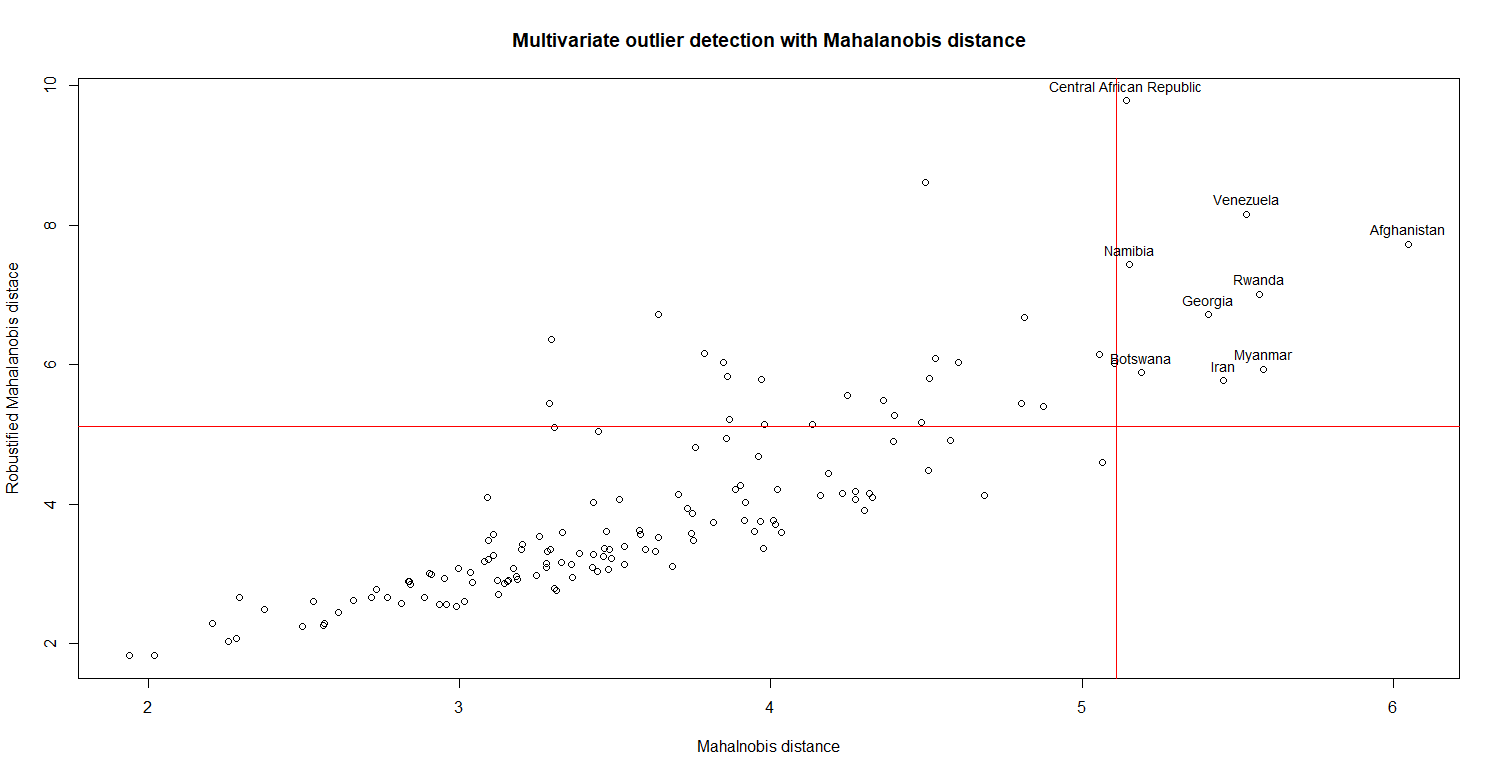
\includegraphics[width=1
    \textwidth]{figures/mahalanobis.png}
    \caption{Plot of regular mahalanobis distance of data points against robustified mahalanobis, with the labels of the data points outside of the cutoff red lines.\label{fig:mahalanobis}}
\end{figure}

For the density-based detection we used the Local Outlier Factor method to give each data point an outlier score depending on the distances with its neighbours and their distances with their own neighbours. We then set a threshold of outlier scores and consider the points above this threshold outliers. In our case, we chose the threshold 1.4 as the majority of the points have a lower score. Another method would be to take the mean of the scores as a threshold, but we consider that it was too low for our data (leaving many points as outliers). The following graph illustrates the outlier scores of our points with the threshold and the labels for the outlier points. We can observe some countries that were also outliers in the previous approach (like Venezuela or Afghanistan), although this time we don’t have the intuition of countries with conflict. In general, these countries can be interpreted as data points that do not have many similar countries, that would be close neighbours. In that sense, we do not consider them as outliers.

\begin{figure}[H]
  \centering
    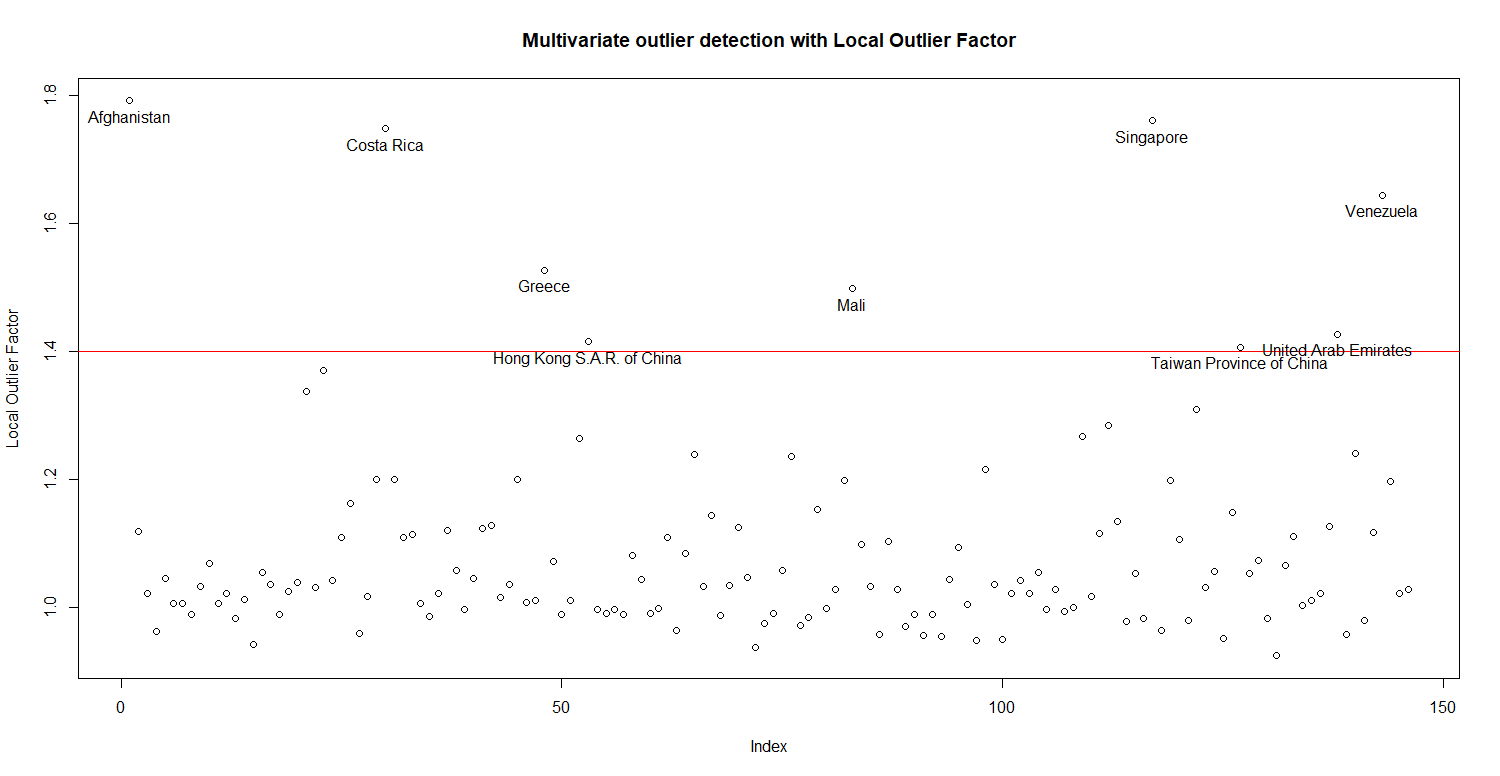
\includegraphics[width=0.90\textwidth]{figures/lof.png}
    \caption{Plot of local outlier factor of the data points, with outlier score threshold as a red line and the labels of the outlier points.\label{fig:lof}}
\end{figure}

\section{Validation Protocol}

Considering our goal is to predict the happiness scores for the different countries, we decided to use as training set the data from 2017, with the added growth variables from 2015-16, and use the 2018 data as test set, removing all instances which have missing values and adding the growth variables for 2016-17. In that way, we can measure the performance of our models by comparing the actual 2018 happiness scores with the predicted ones.

Regarding model validation, we will comment on it and on the model selection method in the following sections.

\newpage
\section{Multivariate Exploration}

In the following subsections we proceed with a multivariate exploration analysis by performing feature extraction, with the subsequent interpretation of the extracted features, and clustering using the new variables. Finally, we complete the clustering discussion with the profiling of the obtained clusters in terms of the original variables.

\subsection{PCA}

In this part, we performed normalized PCA in order to reduce the dimensionality space, perform feature extraction and understand the relations between the variables. In the figure \ref{fig:pca}, we can see that the first principal component explains about 36\% of the total variation, and the second principal component an additional 17.8\%, having a total of 53.8\%.

By looking to the projection of the variables into the PCs, we can see that the first dimension seems correlated to \textit{Happiness.score} and \textit{Negative.affect}. We can interpret it as a dimension which represents happiness versus sadness. In the same way,  the second dimension is highly correlated to \textit{Govern.confidence} and \textit{Growth1}, while slightly correlated  to \textit{Generosity}, \textit{GINI.household.income}, \textit{Freedom.choice} and \textit{Positive.affects}. Thus, we can say this dimension represents how embracing societies are according to people’s perceptions, both in equality, confidence, generosity or freedom.

Overall, we see the bigger contributions to the first factorial plane are the \textit{Happiness.score}, \textit{Log.GDPpc}, \textit{HALE}, \textit{Social.support} and \textit{Freedom.choice}.

\begin{figure}[H]
  \centering
    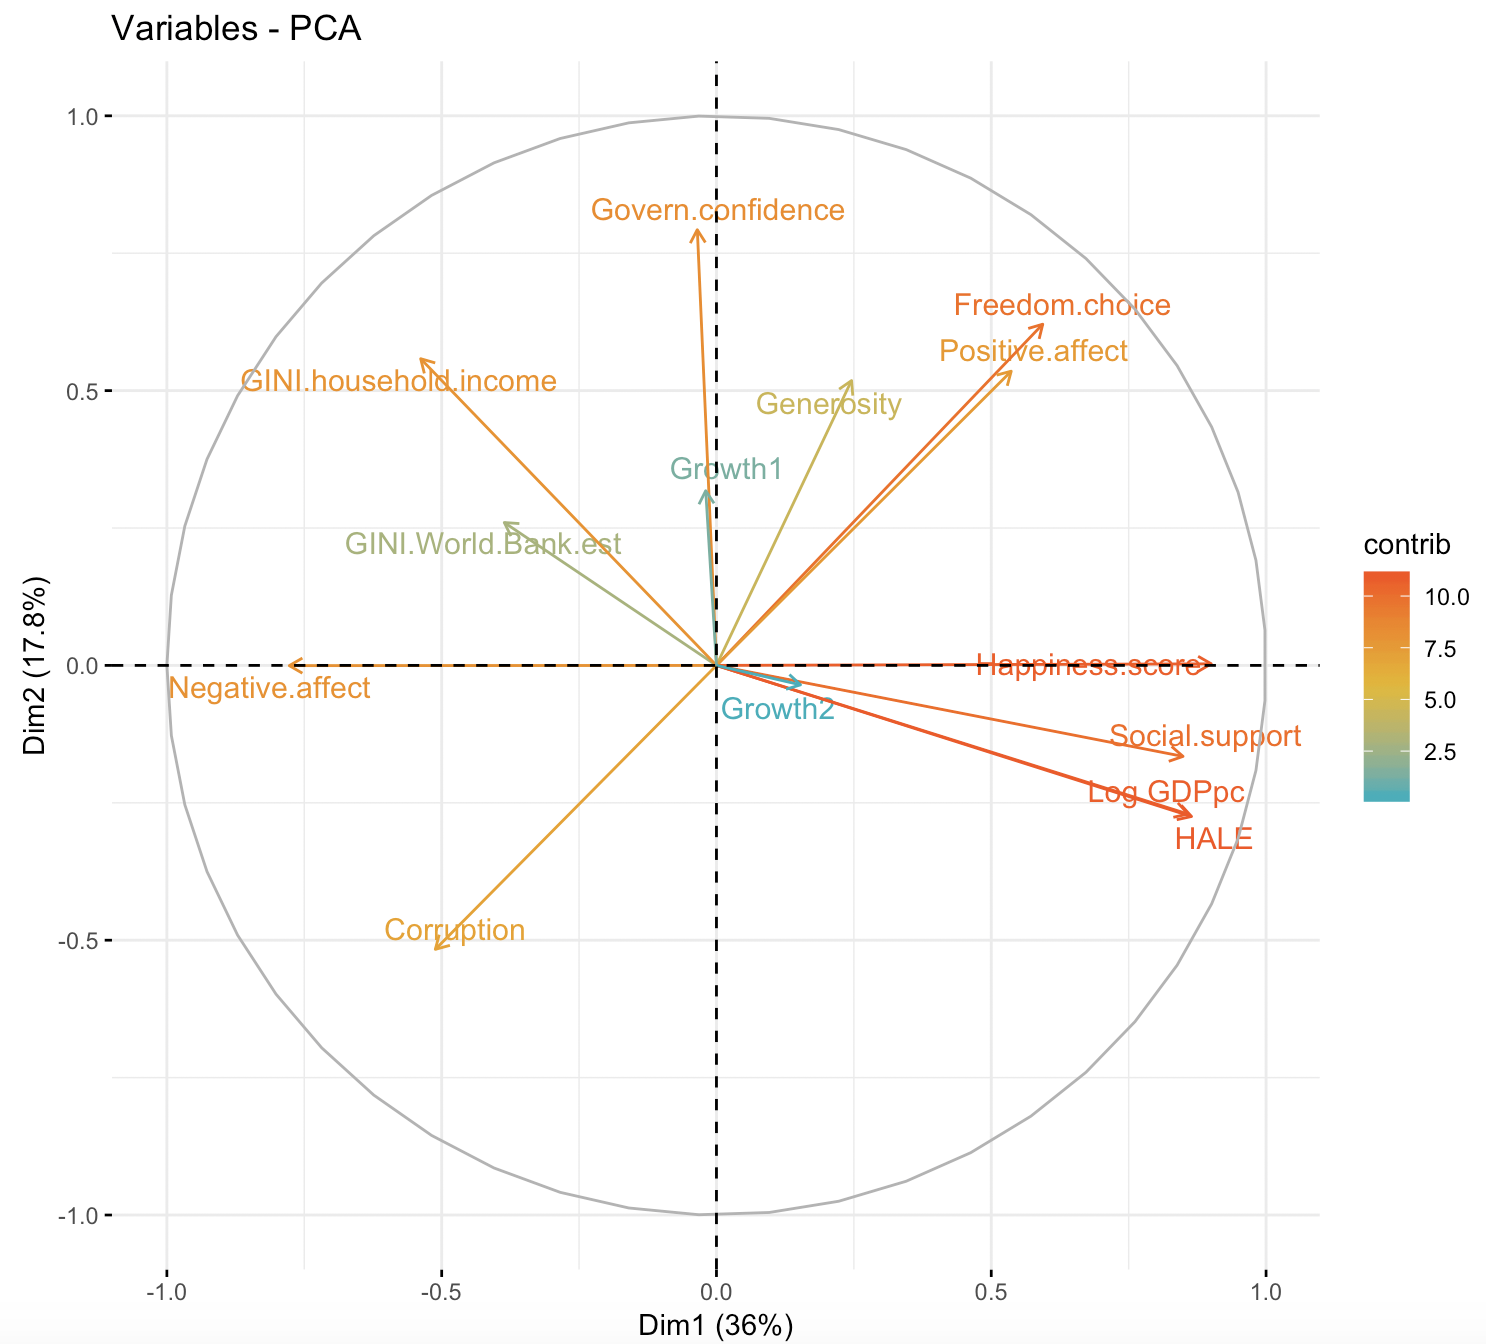
\includegraphics[width=0.85\textwidth]{figures/pca_var.png}
    \caption{Projected variables in the first factorial plane, with color coded contributions for each.\label{fig:pca}}
\end{figure}

In addition, the variable factor map chart shows other interesting facts about our variables. For instance, \textit{Freedom.choice}, \textit{Generosity} and \textit{Positive.affect} seem to be inversely correlated with \textit{Corruption}, so the higher the corruption, the smaller the feeling of freedom, generosity or frequent positive emotions.

\textit{Happiness.score} seem to be inversely correlated to \textit{Negative.affect}, which was to be expected since people who are worried, sad and angry cannot be happy. Furthermore, it seems to be highly correlated with \textit{HALE}, \textit{Social.support} and \textit{Log.GDPpc} which points out the most important factors for happiness scores, that are also correlated to one another.

In contrast to what we may have expected, both growth variables seem not to be well represented in the first factorial plane.

Following our analysis, in the figure below we present the projected individuals in the first factorial plane. The figure shows a generally clear separation between regions, although they are not perfectly separable.

\begin{figure}[H]
  \centering
    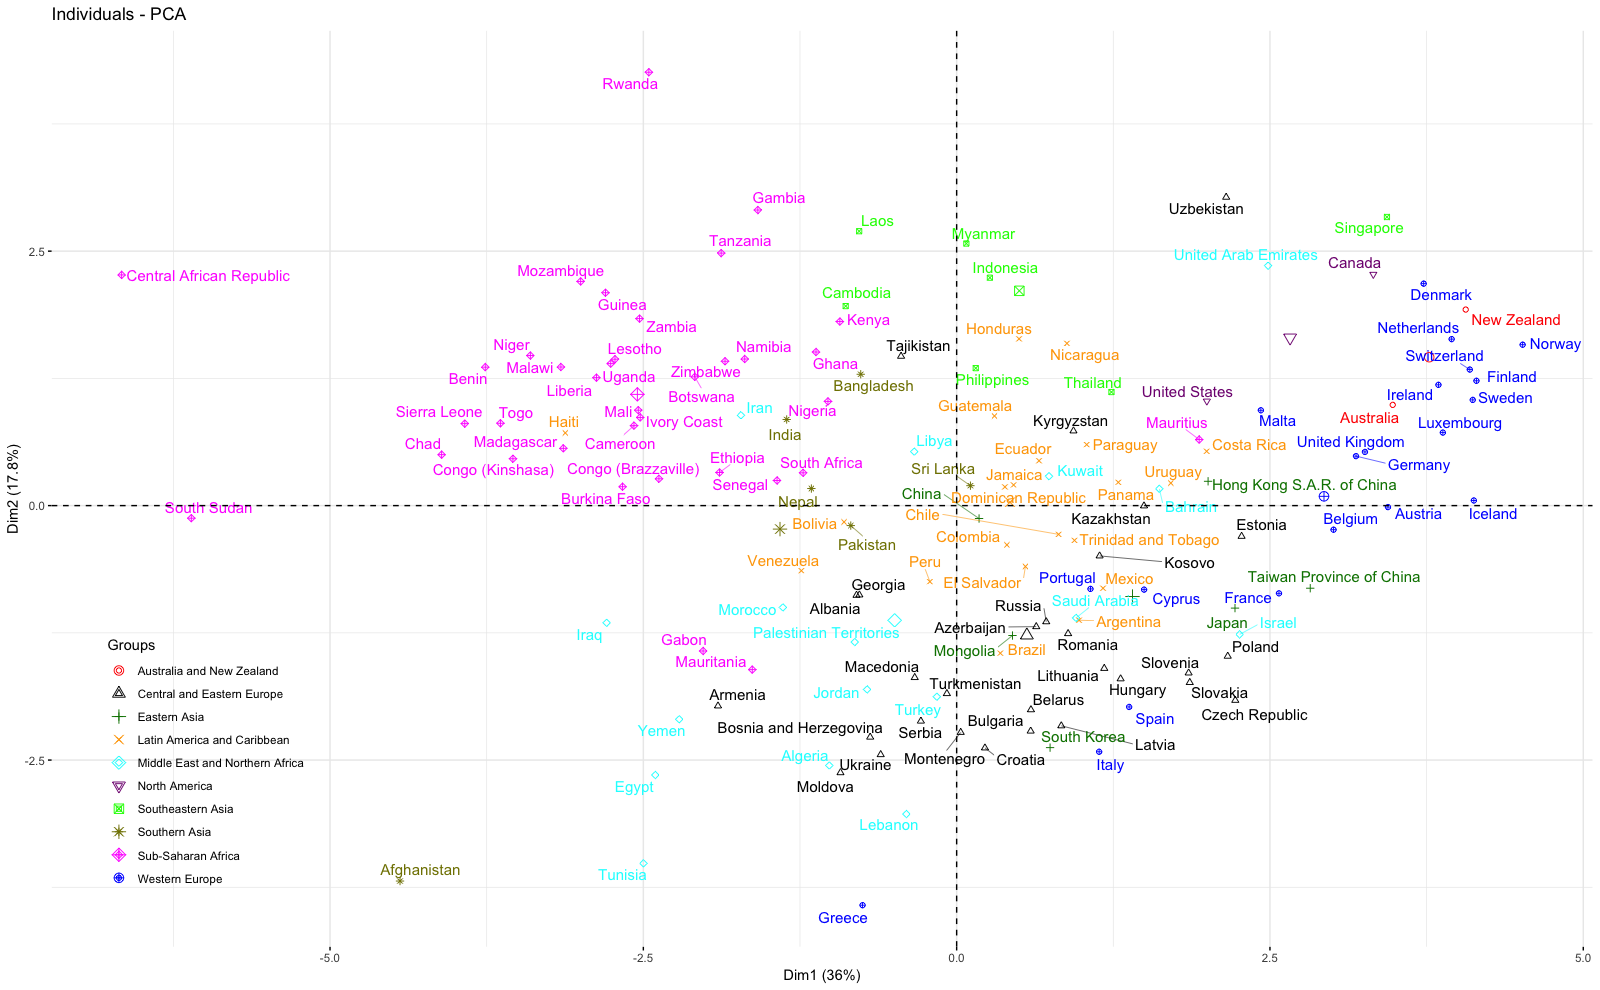
\includegraphics[width=0.85\textwidth]{figures/pca_ind.png}
    \caption{Projected individuals in the first factorial plane with their labels, color coded according to their region\label{fig:pca_ind}}
\end{figure}

We proceed into choosing the right number of significant components. By using the Kaiser rule, taking the PCs that have eigenvalue greater than the mean eigenvalue, represented in the plot by the red dashed line, we should take 5 components. In addition, using also the last elbow criteria we end with 5 components too. Finally, we see that using 5 components we have a total cumulative explained variance ratio of 79.38\%, close to 80\% of explained variance. We conclude the significant principal components are the first 5 PCs.

\begin{figure}[H]
  \centering
    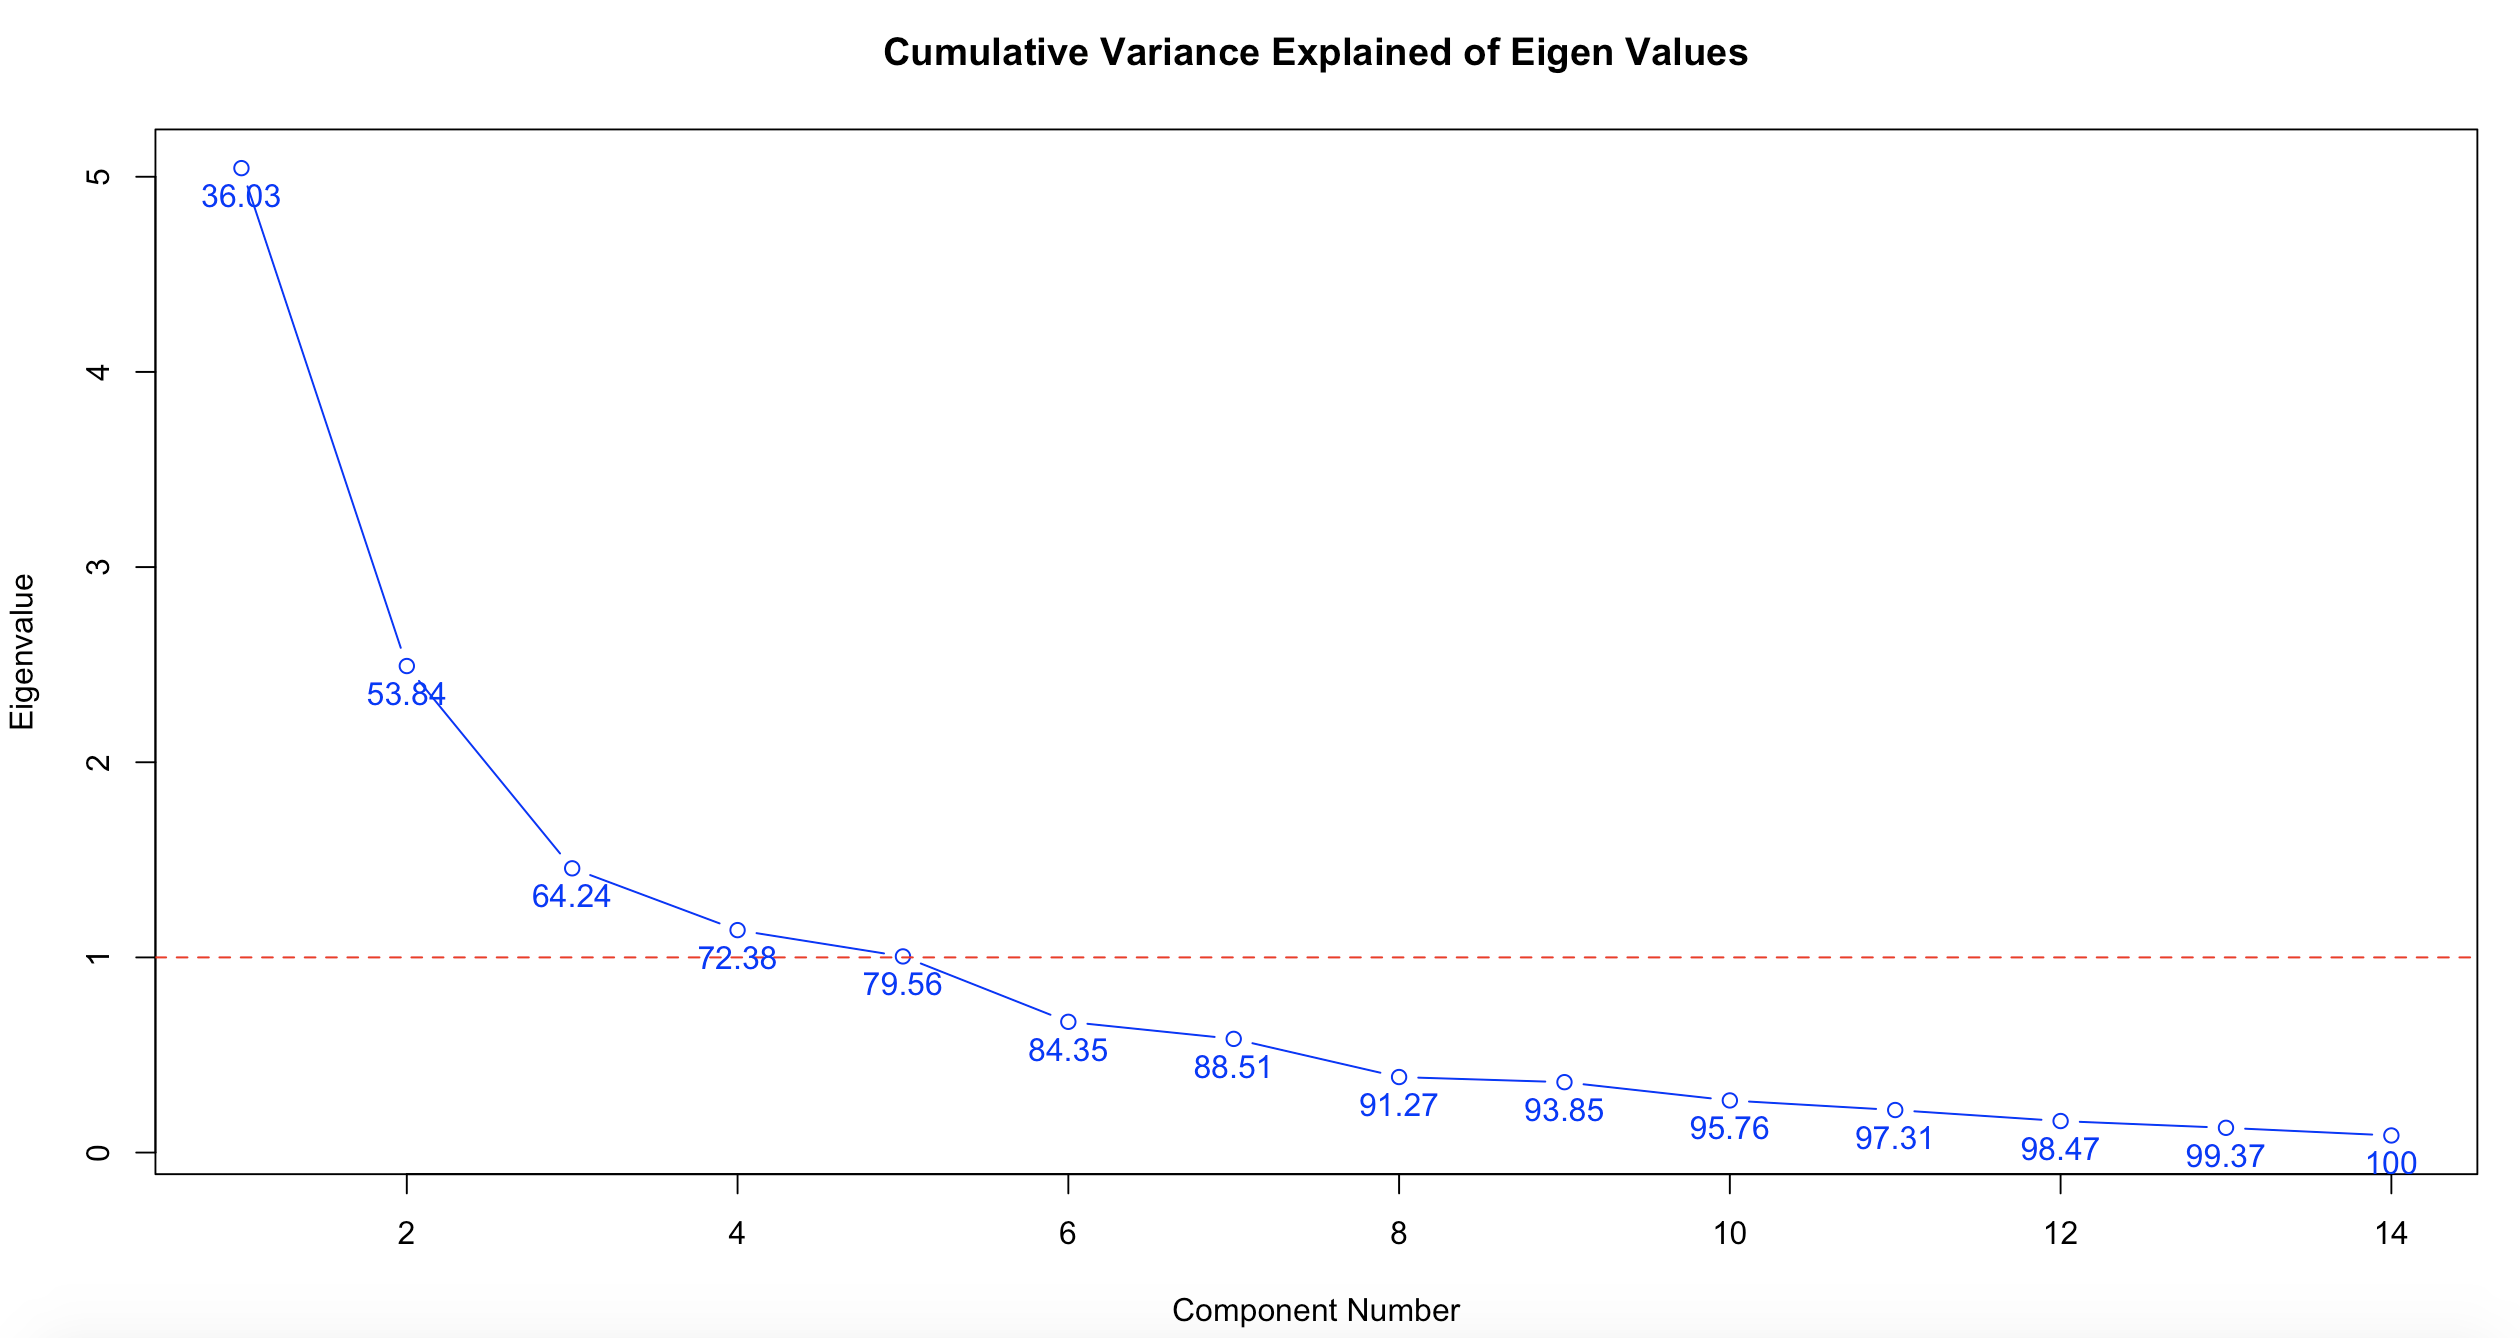
\includegraphics[width=0.85\textwidth]{figures/pca_eigenvalue.png}
    \caption{Explained variance for each principal component, with the labels showing the cumulative explained variance ratio, with red line showing mean eigenvalue.\label{fig:pca_ind}}
\end{figure}

\subsection{Clustering}

After the principal component analysis explained in the last section, we continued with hierarchical cluster analysis in order to group our individuals (countries) with the same characteristics. using ward aggregation method. For this goal we calculated the distances between individuals using euclidean distance.

To choose the right number of clusters, we use the Calinski-Harabass index, as we can see in the figure below, with and without consolidation, the C-H index suggests 4 clusters.

\begin{figure}[H]%
    \centering
    \subfloat[CH index with consolidation]{{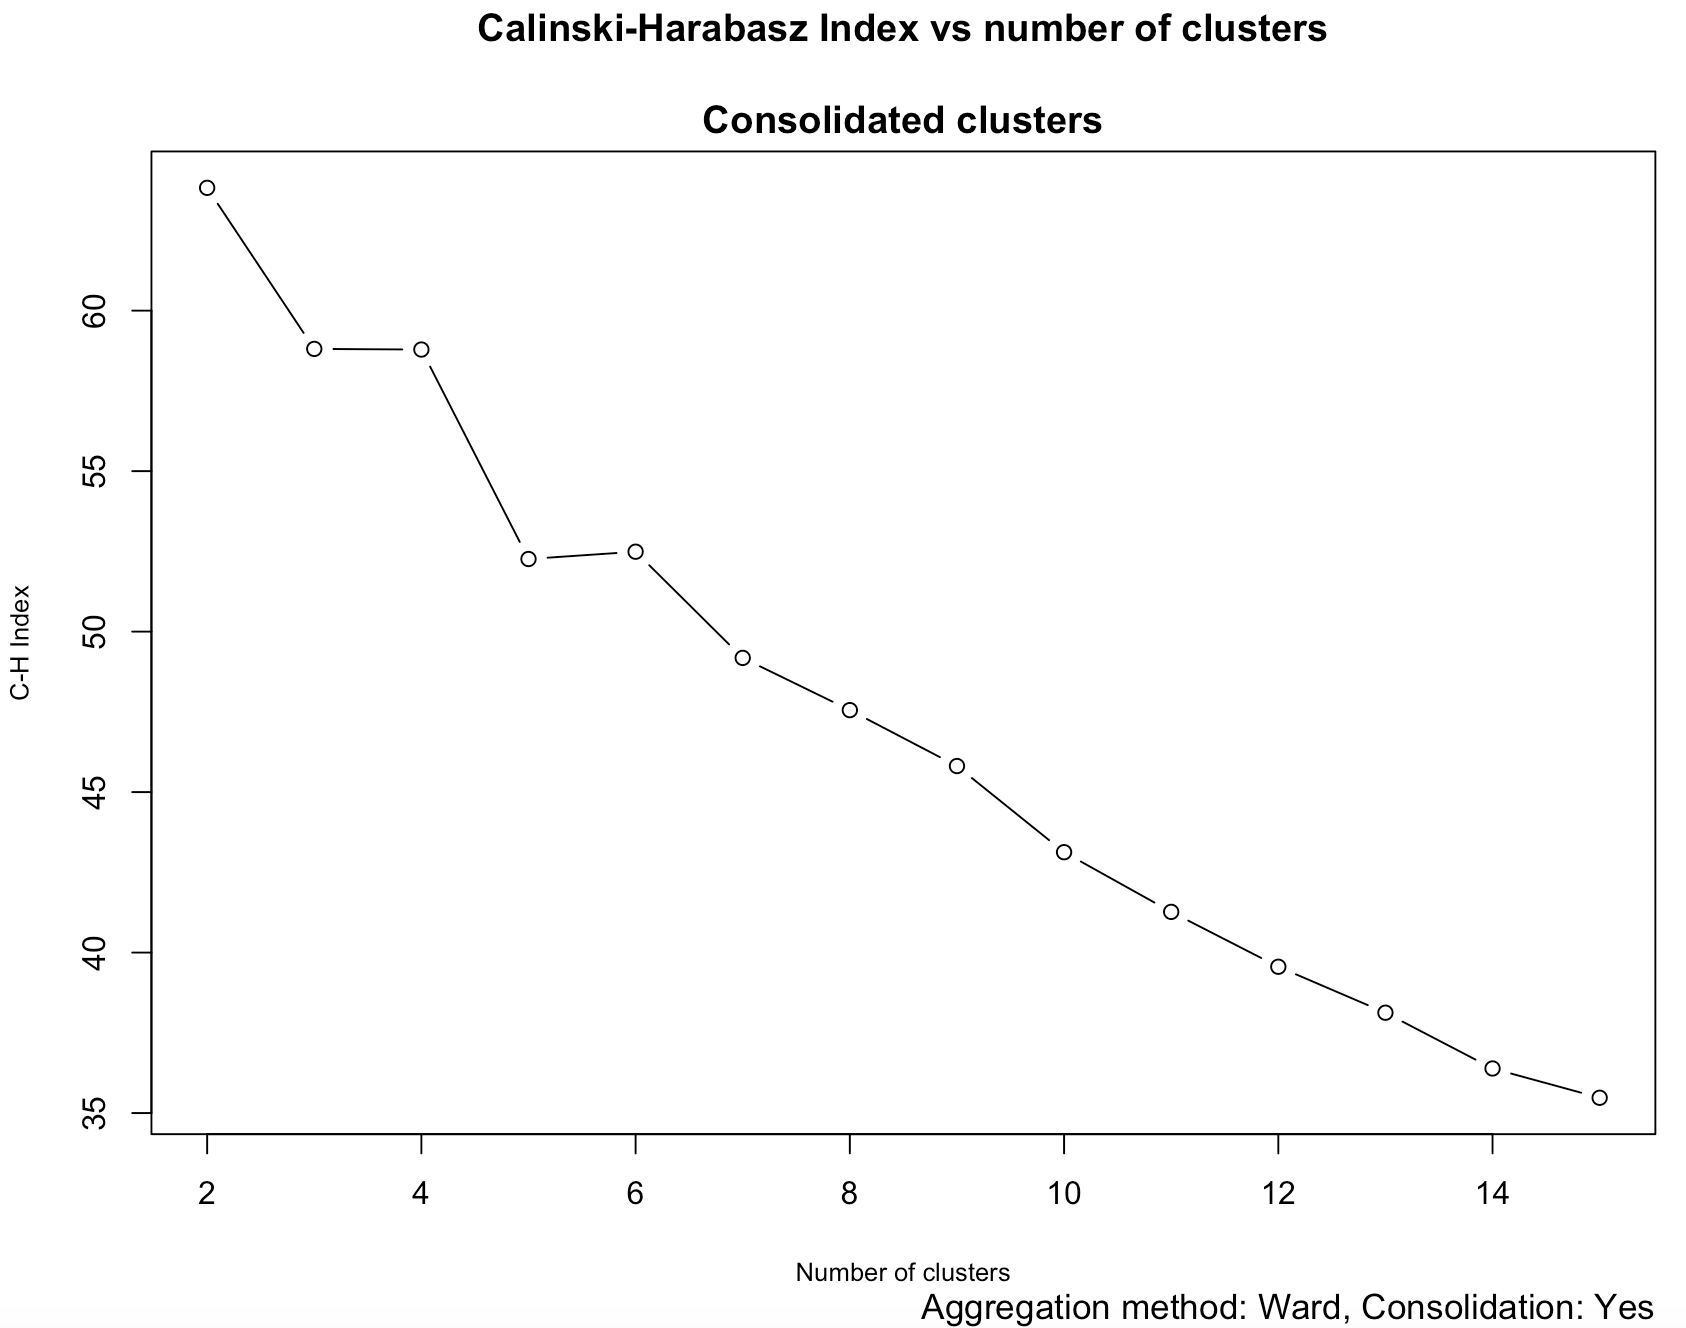
\includegraphics[width=7.5cm]{figures/calinski_consolidation.png} }}%
    \qquad
    \subfloat[CH without consolidation]{{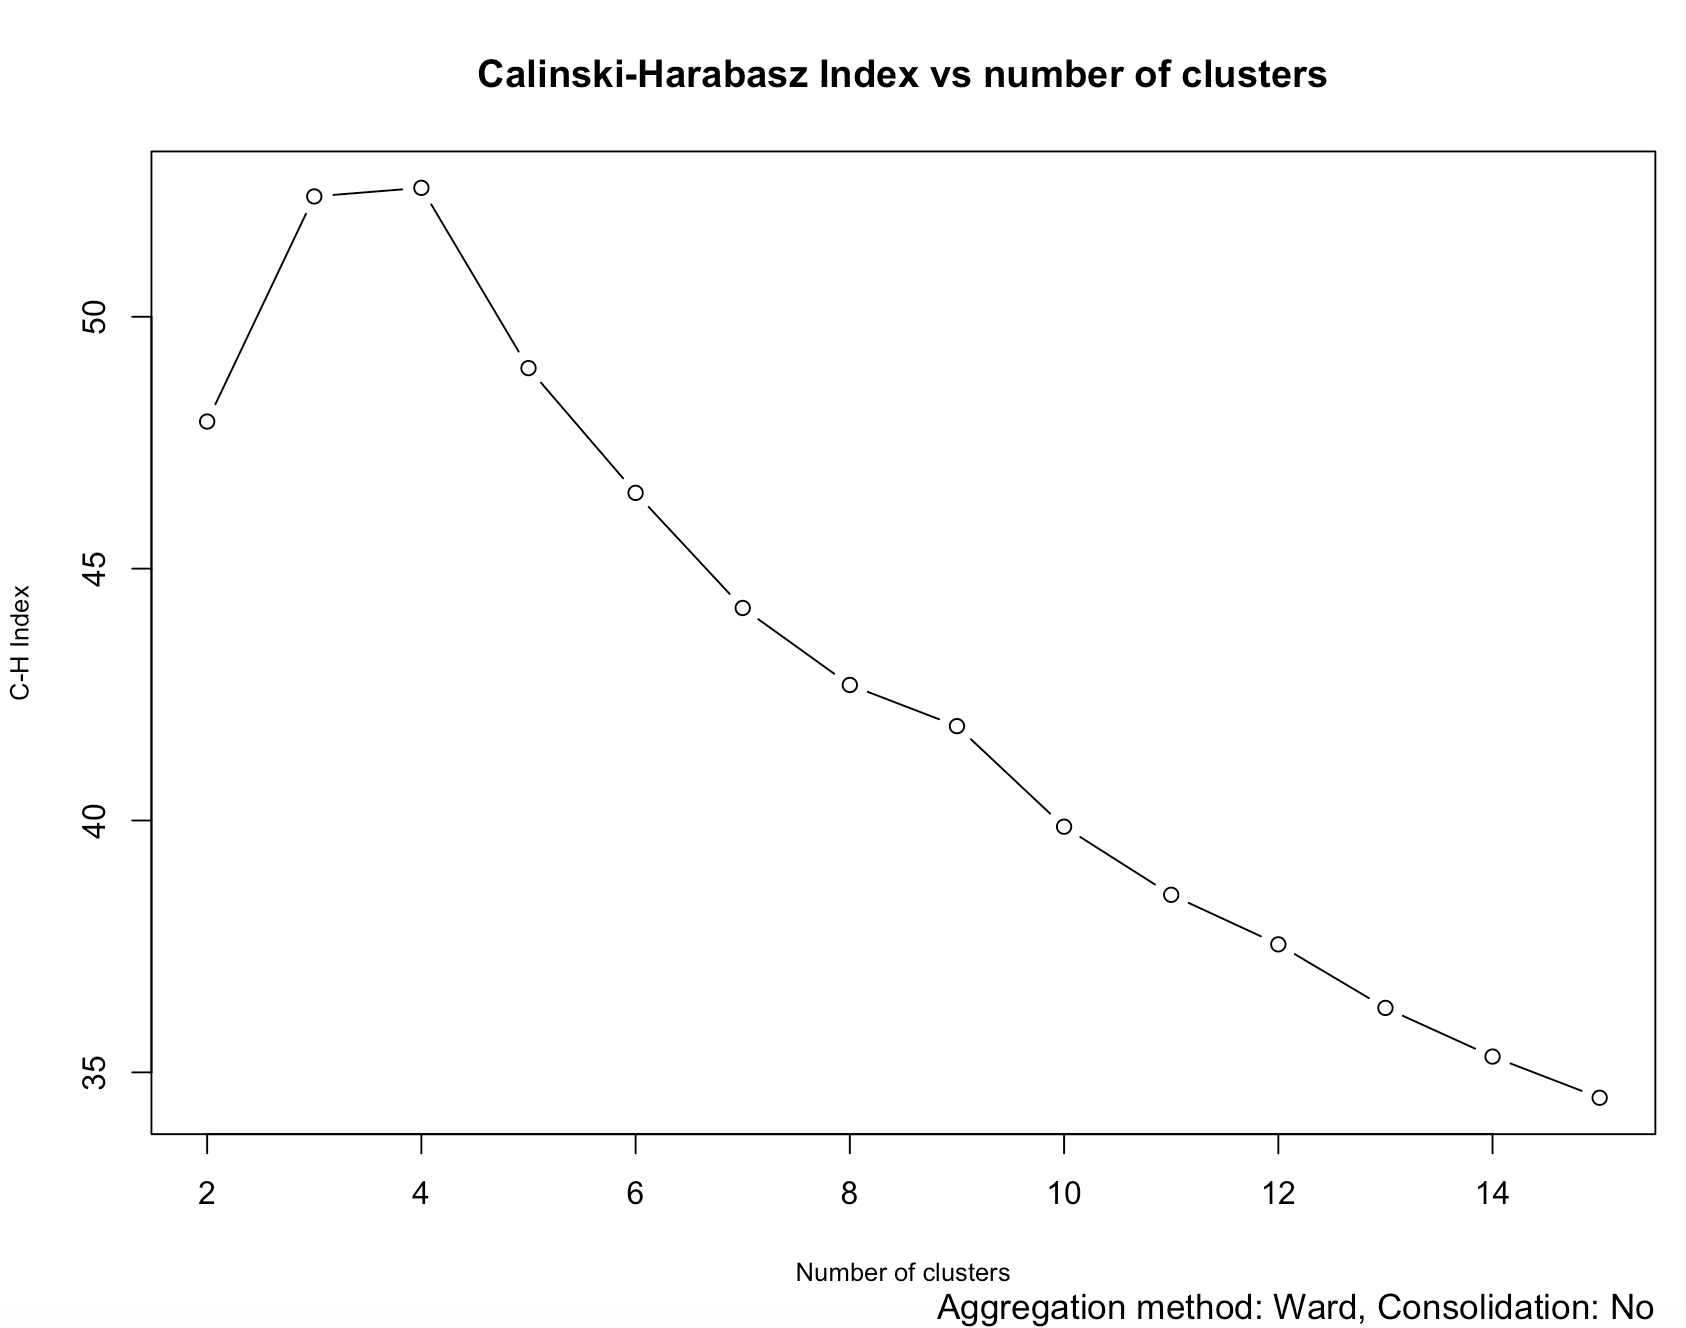
\includegraphics[width=7.5cm]{figures/calinski_no_consolidation.png} }}%
    \caption{Calinski-Harabass index for clustering with different cluster numbers a) with consolidation and b) without consolidation.}%
    \label{fig:example}%
\end{figure}

In the figure below, we can see the dendrogram with 4 clusters.

\begin{figure}[H]
  \centering
    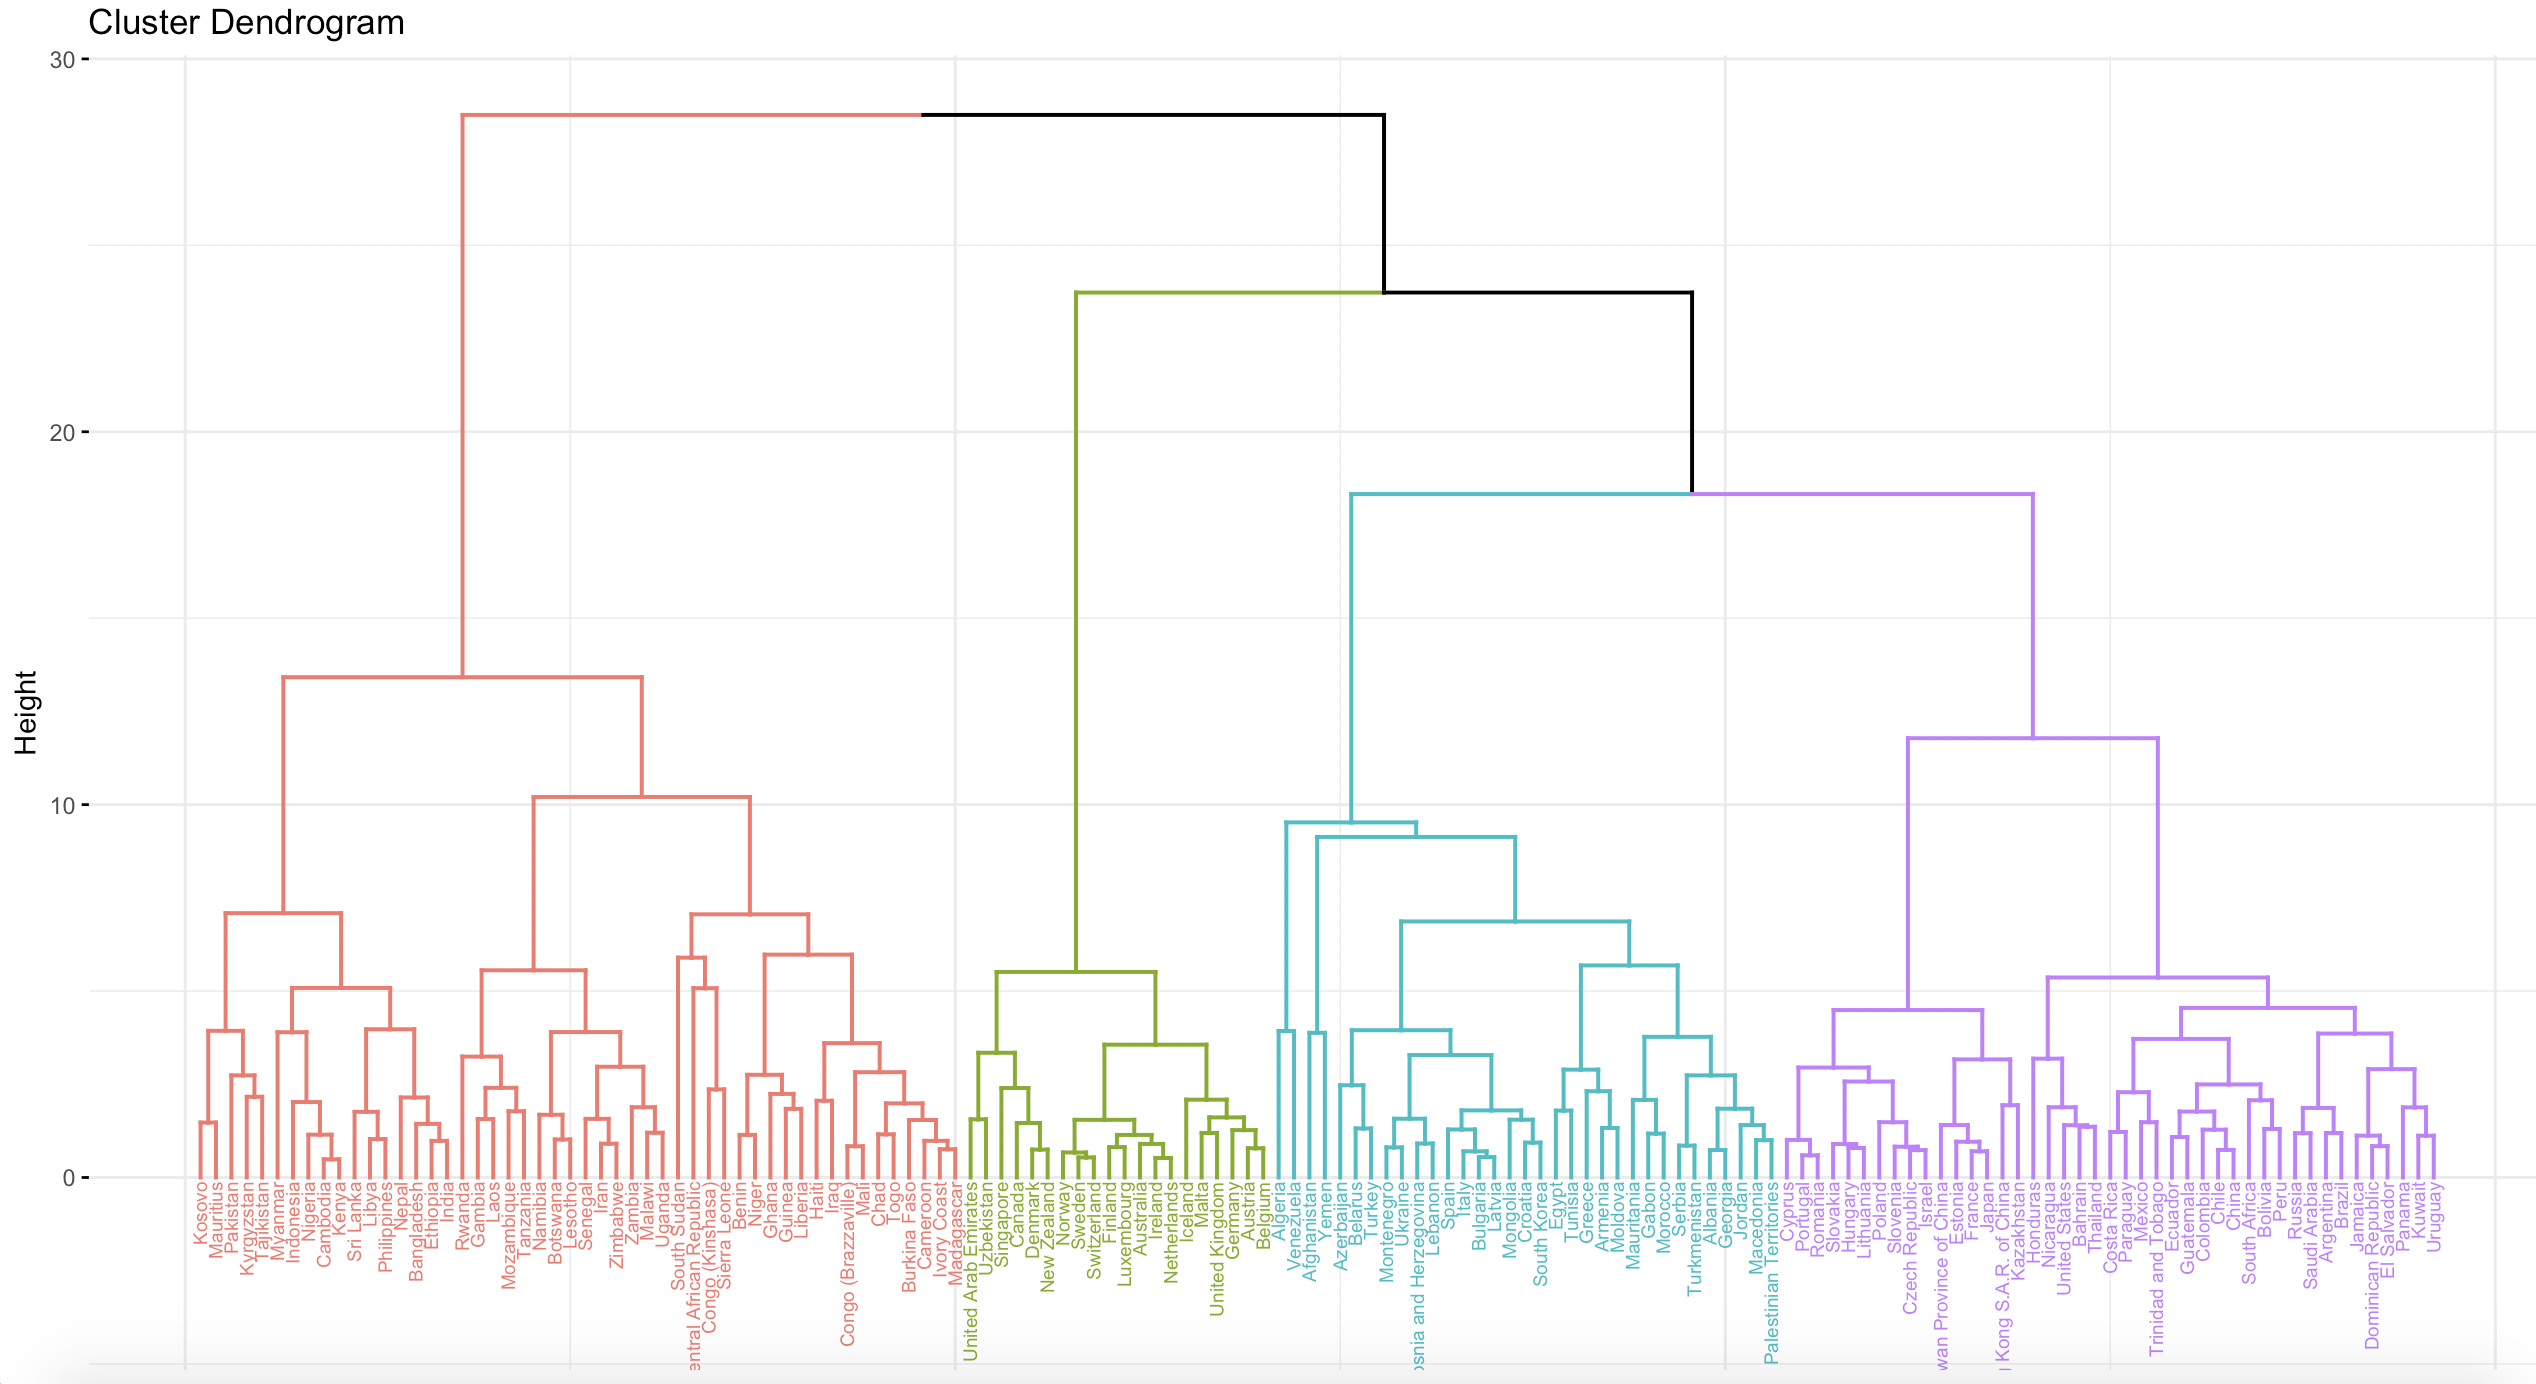
\includegraphics[width=0.85\textwidth]{figures/hierchical_clustering_dendogram.png}
    \caption{Hierarchical clustering dendogram color coded with 4 clusters. \label{fig:pca_ind}}
\end{figure}

Lastly, we proceed to the profiling of the obtained clusters in relation to the original variables. By using the \textit{catdes} function we can see which variables are better represented in each cluster in order to interpret them. 

With regards to the categorical variable \textit{Region}, we see that some clusters clearly represent some regions. We plot the projected individuals with their assigned custer in the factorial plane to better represent them. For instance, we see that cluster 4 significantly represents countries from the \textit{Sub-Saharan Africa} region, while cluster 3 contains most of the countries from \textit{Western Europe} and \textit{Australia} and \textit{New Zealand} regions. In contrast, for cluster 1 we have \textit{Central and Eastern Europe} and the \textit{Middle East} and \textit{Northern Africa} regions and for cluster 2 the \textit{Latin America} and \textit{Caribbean region}, although not so well represented and with countries from other regions.

\begin{figure}[H]
  \centering
    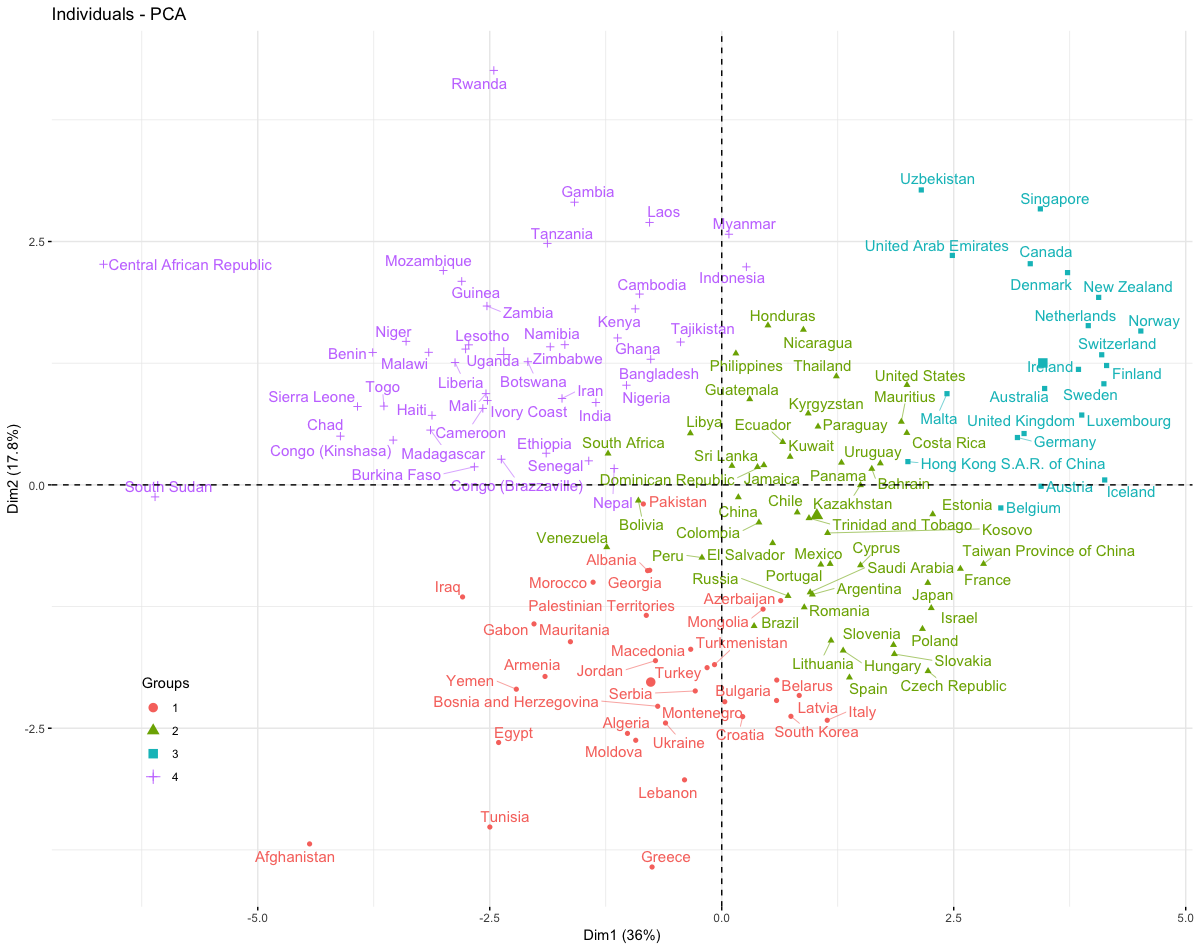
\includegraphics[width=0.85\textwidth]{figures/pca_individuals_clustering.png}
    \caption{Projected individuals in the first factorial plane color coded according to previous 4-cluster clustering.\label{fig:pca_ind}}
\end{figure}

In contrast, for the continuous variables we have the following representations:

\begin{itemize}
    \item Cluster 1 are the countries that have a greater mean than the overall for \textit{Corruption} and \textit{Negative.affect} variables, together with a lower mean in \textit{Happiness.score}. With these, we conclude that people in these countries have a more negative perception of their governments and overall lower happiness
    \item Cluster 2 are countries that, considered through their means,  have slightly higher values of \textit{Social.support}, \textit{Positive.affect}, \textit{Happiness.score} and \textit{HALE} than the population mean. We conclude that these are countries that have generally good consideration of their societies with an overall good happiness score.
    \item Cluster 3 are countries with a much higher \textit{Happiness.score} than the overall mean together with high means in \textit{Log.GDPpc}, \textit{Generosity} and \textit{HALE}. Therefore, this countries have a very good consideration of their societies and accordingly good happiness scores.
    \item Cluster 4 have higher values than the population’s mean in \textit{GINI.household.income} and \textit{GINI.World.Bank.est}, which means more inequality, together with higher \textit{Negative.affect}. However, they also have slightly higher \textit{Govern.confidence}. This shows countries with greater inequalities that lead to people with more frequent negative feelings.
\end{itemize}

By comparing both representations, it makes sense for countries in the specified regions to have the characteristics mentioned above for each cluster.

\section{Model prediction and validation}

After concluding with our exploratory analysis on the dataset presented in the previous section, we proceed our discussion with the fitting of the prediction models, evaluation of our performance and obtained results.

We will present two kinds of models: decision trees with recursive splitting and regularization on the number of leaves, and random forest with bootstrap resampling.


\subsection{Decision trees}

For the decision trees, we will use the \textit{rpart} package to build a maximal tree with binary recursive partitioning and then we tune the complexity parameter, which regularizes tree size, to prune the tree into a final prediction model.

For the hyper-parameter tuning we use a 10-fold cross validation method, sampling randomly from the training dataset into 10 folds and iterating over each fold to use as validation sample while we train with the remaining. 

After building both the maximal tree, we get a tree with 11 leaves (10 splits), represented in the following diagram.

\begin{figure}[H]
  \centering
    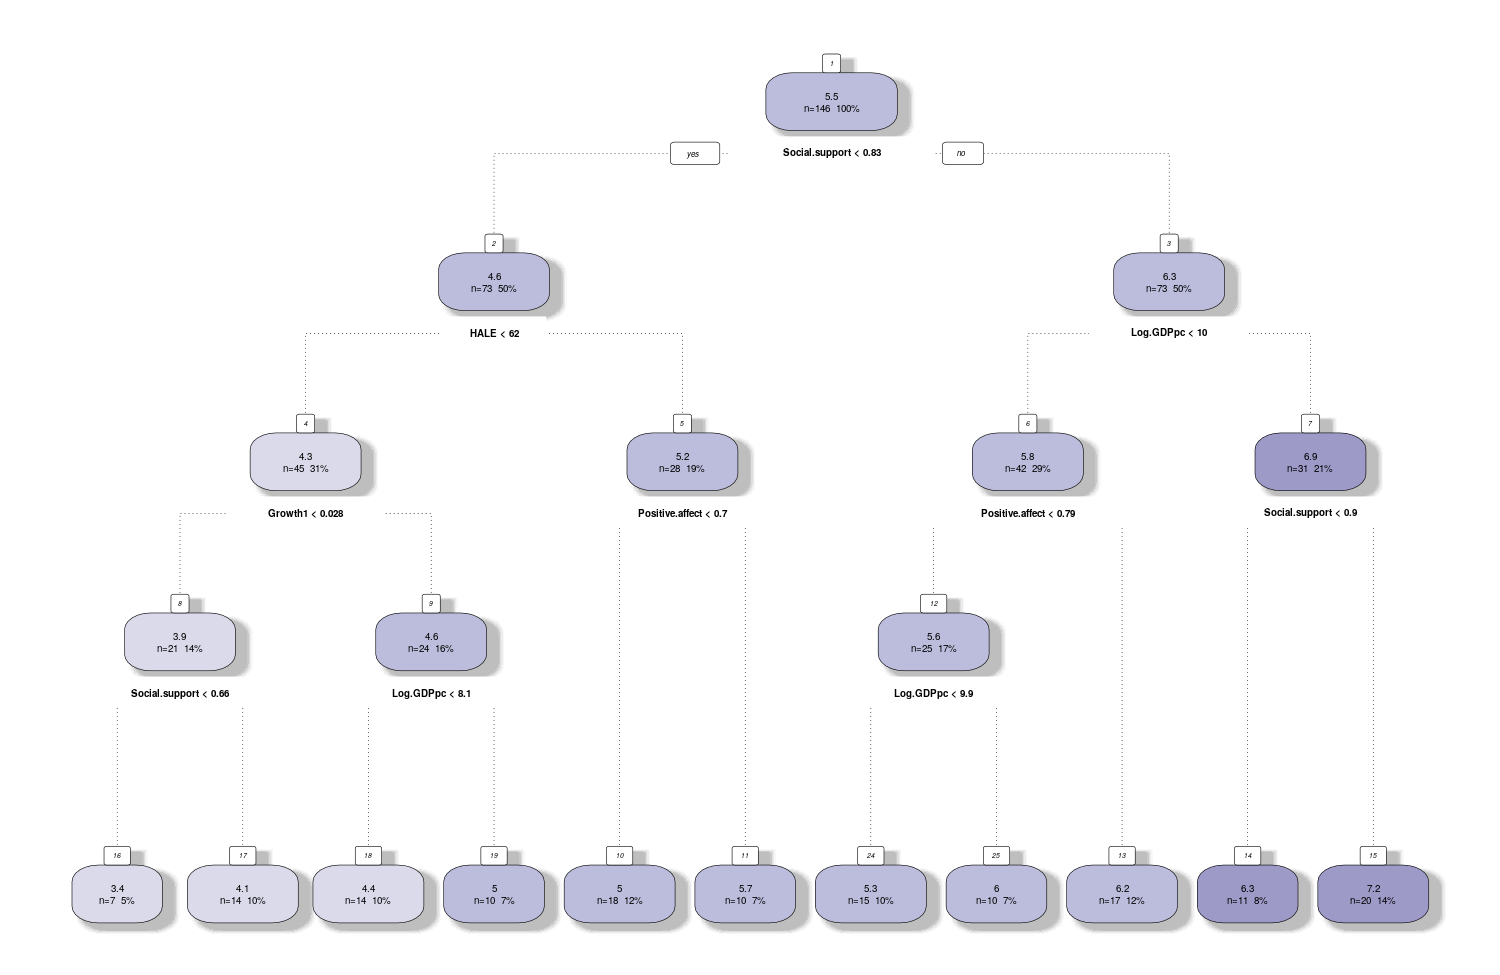
\includegraphics[width=0.85\textwidth]{figures/tree.png}
    \caption{Maximal binary recursively splitting decision tree for the regression model.\label{fig:tree}}
\end{figure}

We see the first split focuses on Social.support while the second and third on \textit{HALE} and \textit{Log.GDPpc}, followed by subsequent splits on the previous variables together with \textit{Positive.affect} and \textit{Growth1}. Note that these variables were the ones that appeared more correlated to \textit{Happiness.score} in the PCA variable analysis, so it makes sense that they are good predictors.

From the \textit{rpart} function we used to build the tree we can get the error for each pruned subtree, by pruning at each split, using 10-fold cross validation, and we can plot this error against the number of leaves in the following chart:

\begin{figure}[H]
  \centering
    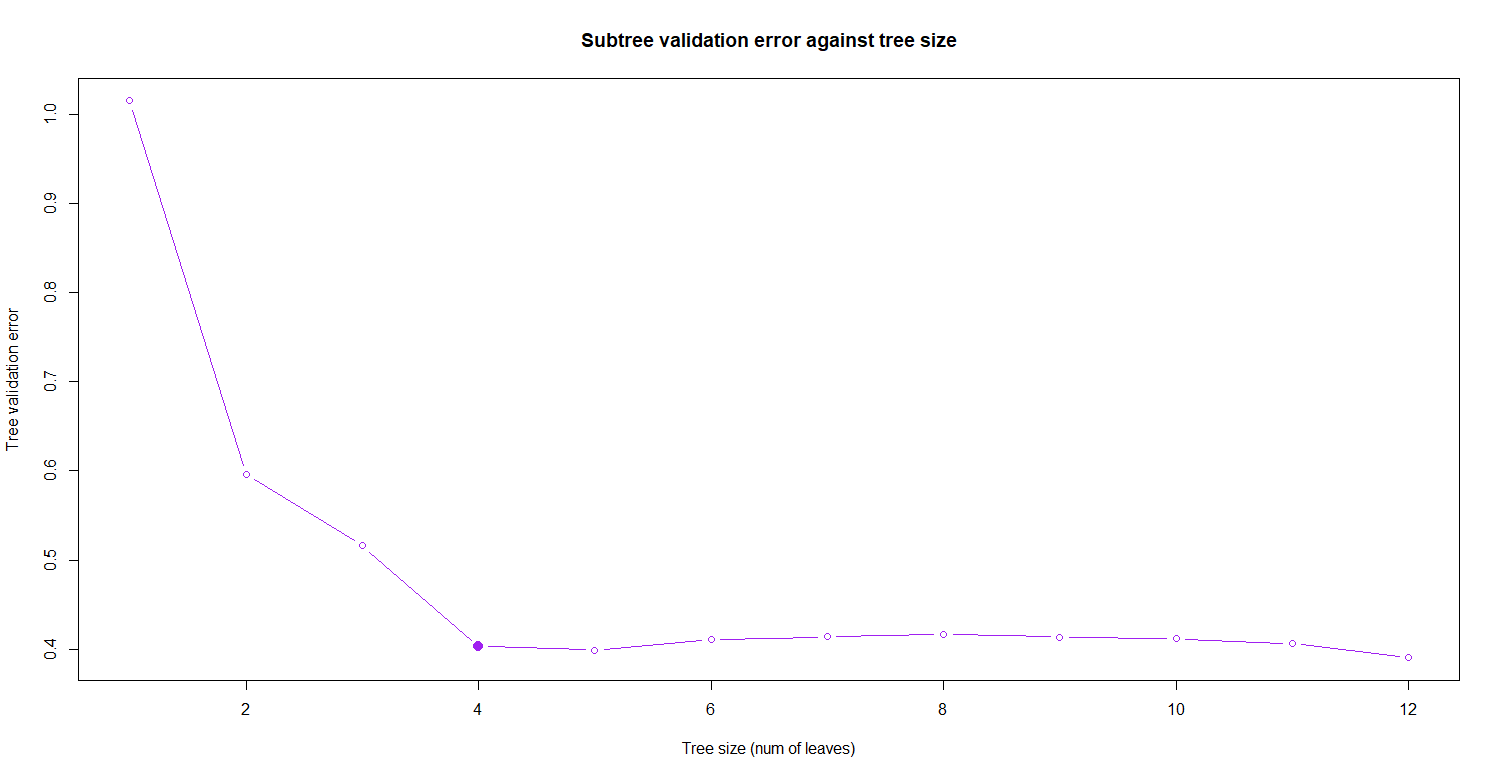
\includegraphics[width=0.85\textwidth]{figures/tree-error.png}
    \caption{Decision tree error against size of tree, as number of leaves, with the optimal decision tree size as filled data point.\label{fig:tree_error}}
\end{figure}

The chart includes a marked point that corresponds to the minimum size tree which has an error lower than the minimum error plus 1 standard deviation. This relaxation from the minimum error tree is taken to build a more prudent tree. We prune the maximal tree with the complexity parameter that corresponds to this tree size, and get the following tree:

\begin{figure}[H]
  \centering
    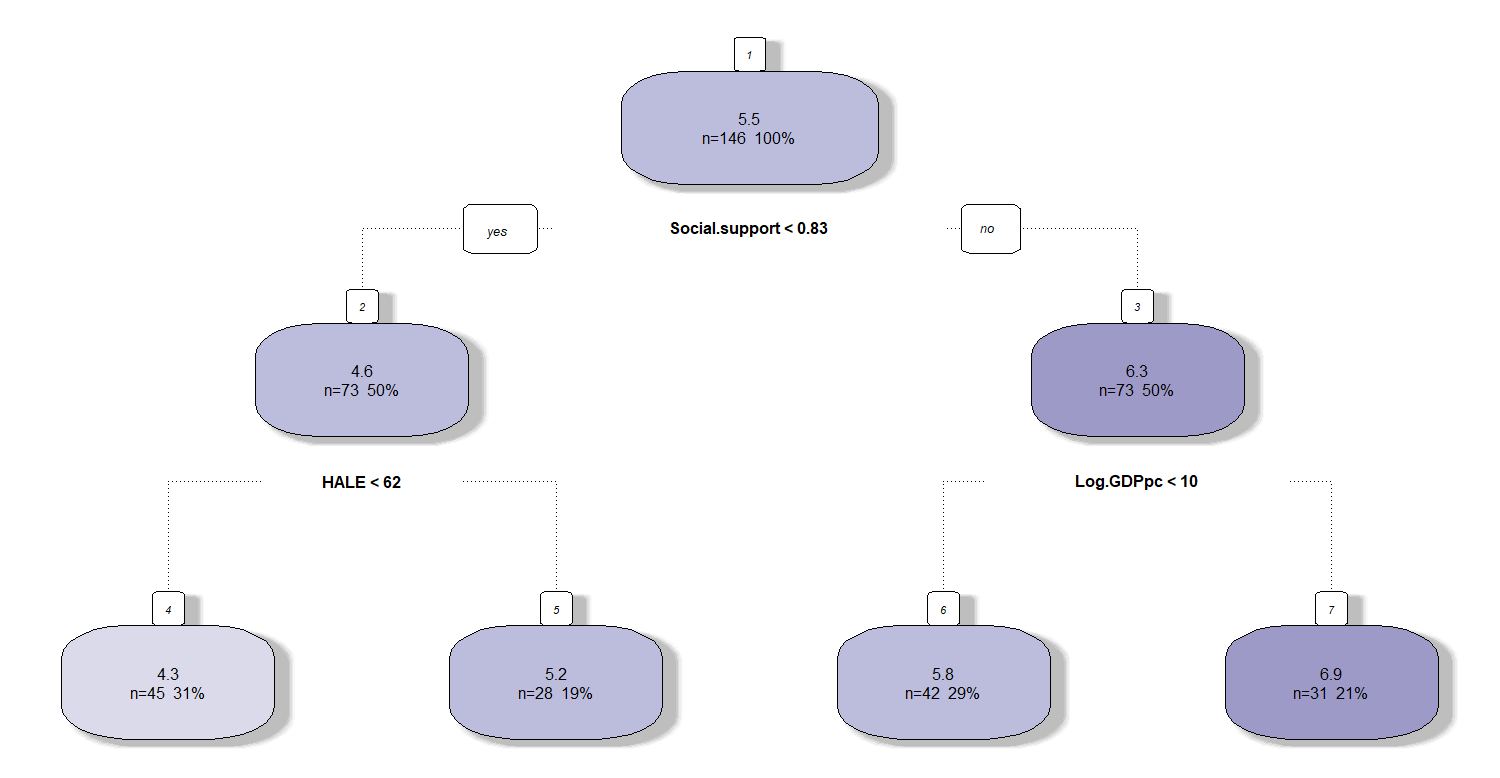
\includegraphics[width=0.85\textwidth]{figures/tree-pruned.png}
    \caption{Pruned decision tree according to optimal complexity parameter.\label{fig:tree_pruned}}
\end{figure}


In the following, we proceed to make predictions on the test 2018 data with both the maximal and the pruned tree, and compare the results. The following plot shows the predicted against the real values for both trees, together with a diagonal straight line showing the perfect predictions.

\begin{figure}[H]
  \centering
    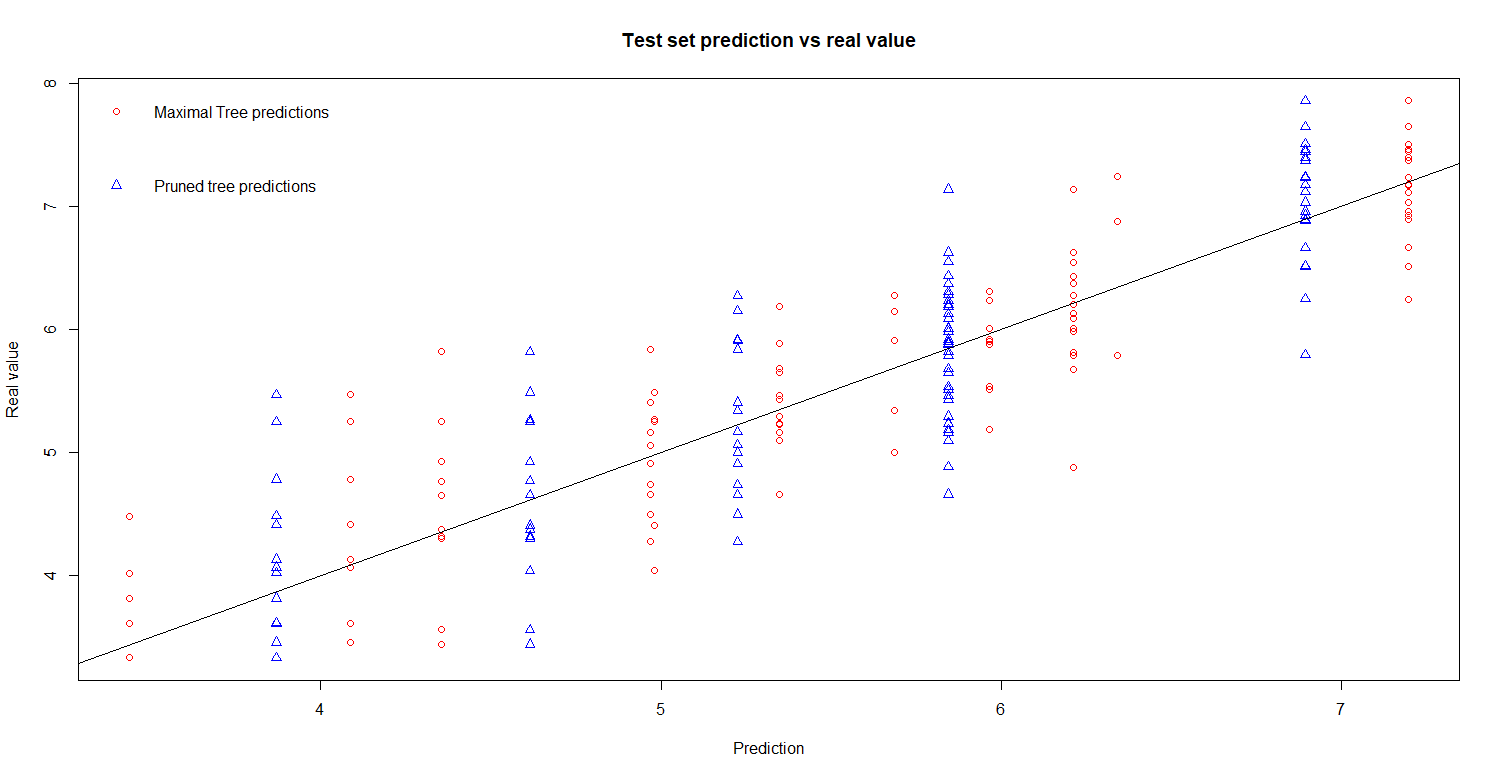
\includegraphics[width=0.85\textwidth]{figures/tree-predict.png}
    \caption{Predicted response variables against real response variables for both the maximal and pruned decision trees\label{fig:tree_predict}}
\end{figure}

Trivially, the maximal tree seems to get closer to the perfect prediction line, as it has more leaves.  What’s more, we see there’s not much difference between the variance of the predicted points with lower and higher happiness scores, which is also bigger for the pruned tree.

In addition to the prediction plot, we can compute the mean square error (MSE) for each tree as a comparative performance measure. We get a MSE of 0.26 for the maximal tree and 0.35 for the pruned tree. In general, the process of pruning makes sense in order to get a smaller tree with almost the same error than a maximal tree. However, we see that our maximal tree performs significantly better than the prune tree. We attribute this to the small size of our tree, which makes the pruning lose too much predictive power. Therefore, we conclude our maximal decision tree is the better decision tree model to predict the happiness scores.


\subsection{Random Forest}

Additional to the decision tree model we presented in the previous section, we proceed to building a random forest model for our data. In order to do so, we use the \textit{randomForest} package in R. We evaluate the resulting performance and we optimize the number of trees, guided by the MSE error.

A random forest is a set of decision trees which are trained with a bootstrapped sample of the data. In addition, in each split of each tree only a random subset of predictors is considered. As we are dealing with a regression problem, we use random subsets of size p/3, with p as the number of predictors (thus 5 for subset in our case). Moreover, the sample with which each tree in the forest is trained is of full size (same size as the training sample) but the sampling method is done with replacement, so an instance can be chosen more than once (bootstrapped samples).

The estimated error of our random forest is 0.1423, much better than with the decision trees. Thus, we obtain a much better model. 

With the same function call of the \textit{randomForest} package, we change the number of predictors of each subset to the full size of predictors, effectively performing bagging without random predictors. The prediction error obtained by the bagged regression trees is \textit{0.1356} which is almost the same with what we obtained with the random forest, although slightly better. We attribute this to the fact that we do not have many predictors and so the random variable subset selection in random forest does not benefit the prediction in a significant way. The following table shows a summary of the model’s errors:

\begin{longtable}[c]{cl}
    \rowcolor[HTML]{C0C0C0} 
    \textbf{Model} & \multicolumn{1}{c}{\cellcolor[HTML]{C0C0C0}\textbf{MSE}} \\\hline \endhead
             Random forest & 0.1466 \\\hline
             Bagged decision trees & 0.1356 \\\hline
    \label{variables}
\end{longtable}

Nevertheless, as bagging does not greatly improve prediction over random forest, we proceed with the random forest model we built. The following chart shows the predictions of both models against the real values, where we can see there’s no appreciable difference between the models.

\begin{figure}[H]
  \centering
    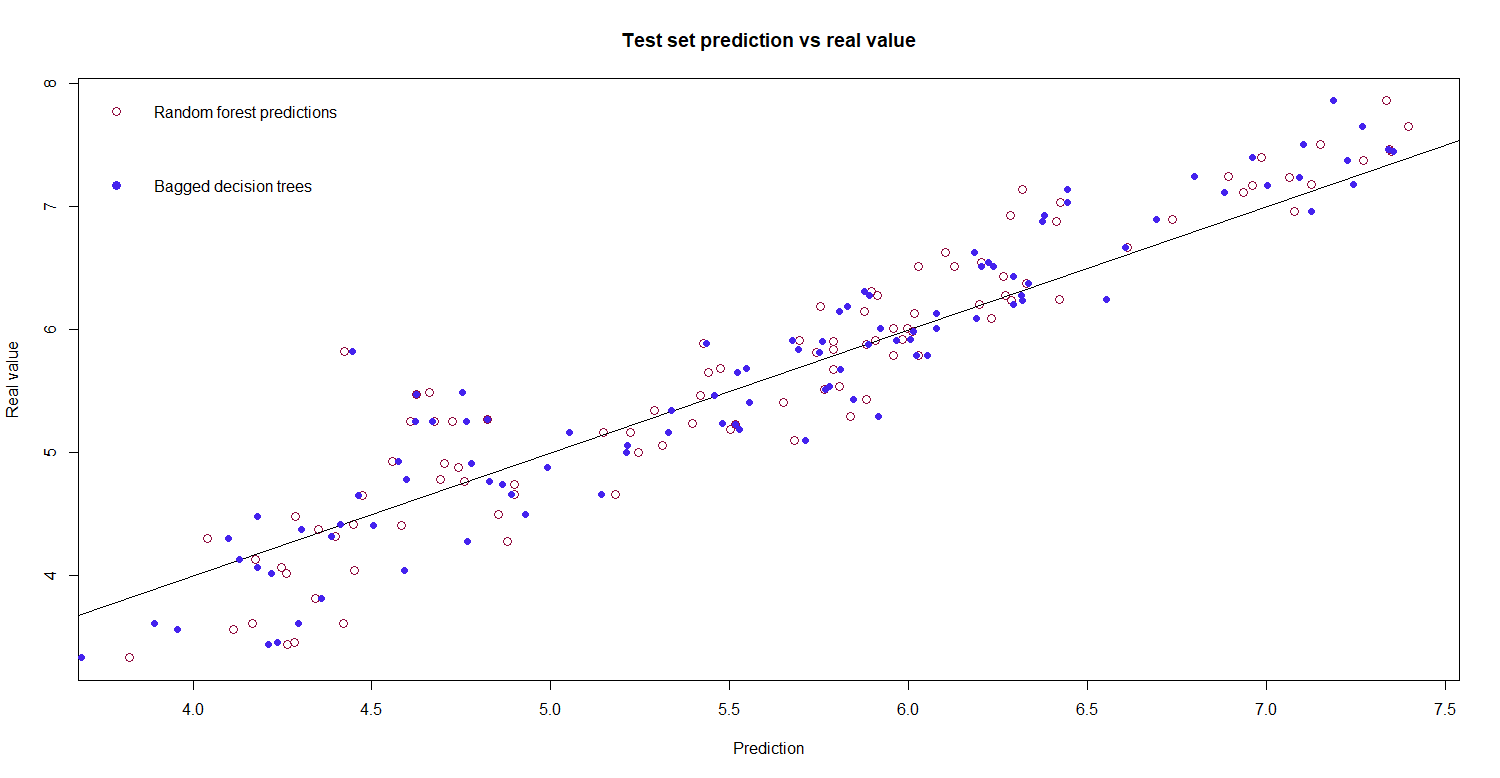
\includegraphics[width=0.85\textwidth]{figures/random-prediction.png}
    \caption{Prediction against real values for random forest and bagged decision trees.\label{fig:random-prediction}}
\end{figure}

Finally, for the construction of our random forest model, we want to ensure that the procedure builds the model using the optimal number of trees. We can tune this parameter by exploring the error we obtain for different number of trees. In the following graph, we illustrate the results we obtained for trying as number of trees values from 1 to 1000, with the mean of each tree’s mean square error for each forest (MMSE):

\begin{figure}[H]
  \centering
    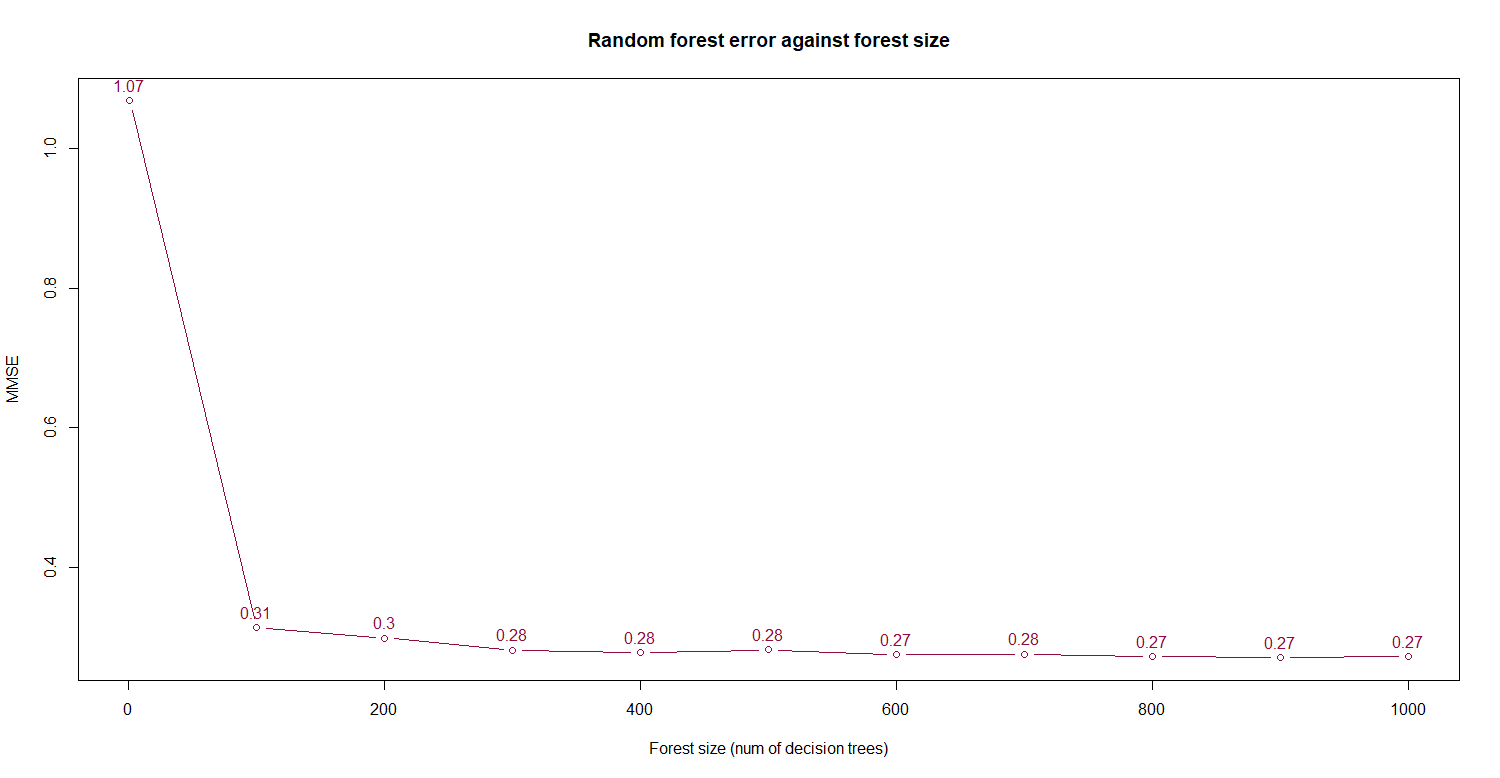
\includegraphics[width=0.85\textwidth]{figures/random-error-size.png}
    \caption{Random forest mean square error vs forest size.\label{fig:random-error-size}}
\end{figure}

The error rate, drops dramatically for values higher than 100. The results show that for a number of 900 trees, we obtain the minimum error rate. However, there difference between 900 and 400 trees is negligible. For that reason, we conclude to use a forest size of 400 trees, as a compromise between low error rate and smaller models (lower computational cost).

As a final step for the construction of the model, we refit the tree with the 400 trees and get a MMSE of \textit{0.1423}. We see that is slightly better than the original random forest, although not significantly. In addition, we still get higher error than the bagged decision trees.

Lastly, we calculate the importance of the variables. The results indicate that across all the trees considered in the random forest, the \textit{Social.support}, \textit{Log.GDPpc} and \textit{HALE} are among the top important variables as we expected from the PCA analysis, followed by Region, which could also be expected from the clustering in the first factorial plane. We can see a chart with the importance of the variables in our random forest.

\begin{figure}[H]
  \centering
    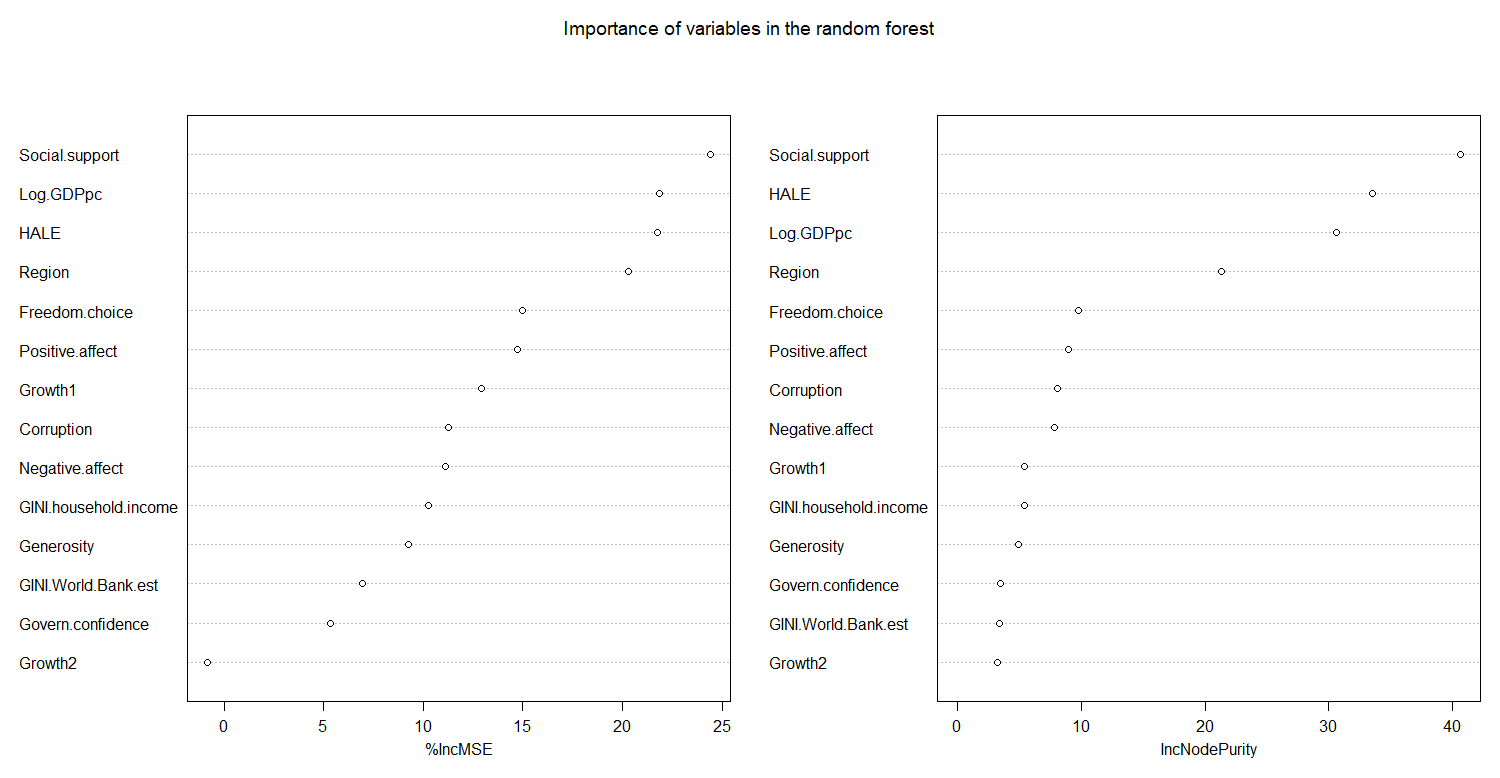
\includegraphics[width=1\textwidth]{figures/random-importance.png}
    \caption{Variables Importance\label{fig:random-importance}}
\end{figure}

\newpage
\section{Conclusions}

In this report we have studied the dataset of the World Happiness Report of 2019, in particular the data from the years 2017-18.

After preprocessing the data to remove unnecessary or poor quality variables and data points, with lots of missing values, we imputed the remaining missing values and performed outlier detection, not finding any significant outlier.

We performed a multivariate exploratory analysis on our dataset in order to extract information from it. The feature extraction through PCA allowed us to have a lower dimension representation, in the first factorial plane, and see the relations between the variables (both the active variables and the supplementary region), in particular between the \textit{happiness scores} and the \textit{social support}, \textit{GDP per capita} and \textit{HALE}. Furthermore, we interpreted the first principal component as a measure of happiness against negative feelings; and the second principal component as a measure of how embracing societies are according to people’s perceptions.

Using the extracted factors we performed clustering with hierarchical clusters and consolidated the results with k-means. By profiling the obtained clusters according to the original variables we could interpret them and found relations between clusters and the perception of society, happiness scores and frequent positive/negative feelings.

Finally, we built prediction models to compute the happiness score depending on the other predictors. We confirmed the best predictors as the ones we saw correlated to the happiness score in the exploratory section.
Specifically, we built a decision tree model and a random forest model, discussing and tuning their parameters, and got estimates on the performance of their predictions. We concluded that the best model was the random forest (together with the bagged decision trees).

\begin{thebibliography}{9}

\bibitem{sachs}
Helliwell, J., Layard, R., \& Sachs, J. (2018)\\
\textit{World Happiness Report 2019}\\
New York: Sustainable Development Solutions Network.

\bibitem{buthan}
Buthan (2012).\\
\textit{\href{https://sustainabledevelopment.un.org/index.php?page=view&type=400&nr=617&menu=35}{Defining a New Economic Paradigm: The Report of the High-Level Meeting on Wellbeing and Happiness}}\\
UN Sustainable Development Knowledge Platform




\end{thebibliography}


\newpage


\begin{landscape}
\thispagestyle{empty}
\section{Appendix: Projected active and supplementary individuals}
\begin{figure}[H]
  \centering
    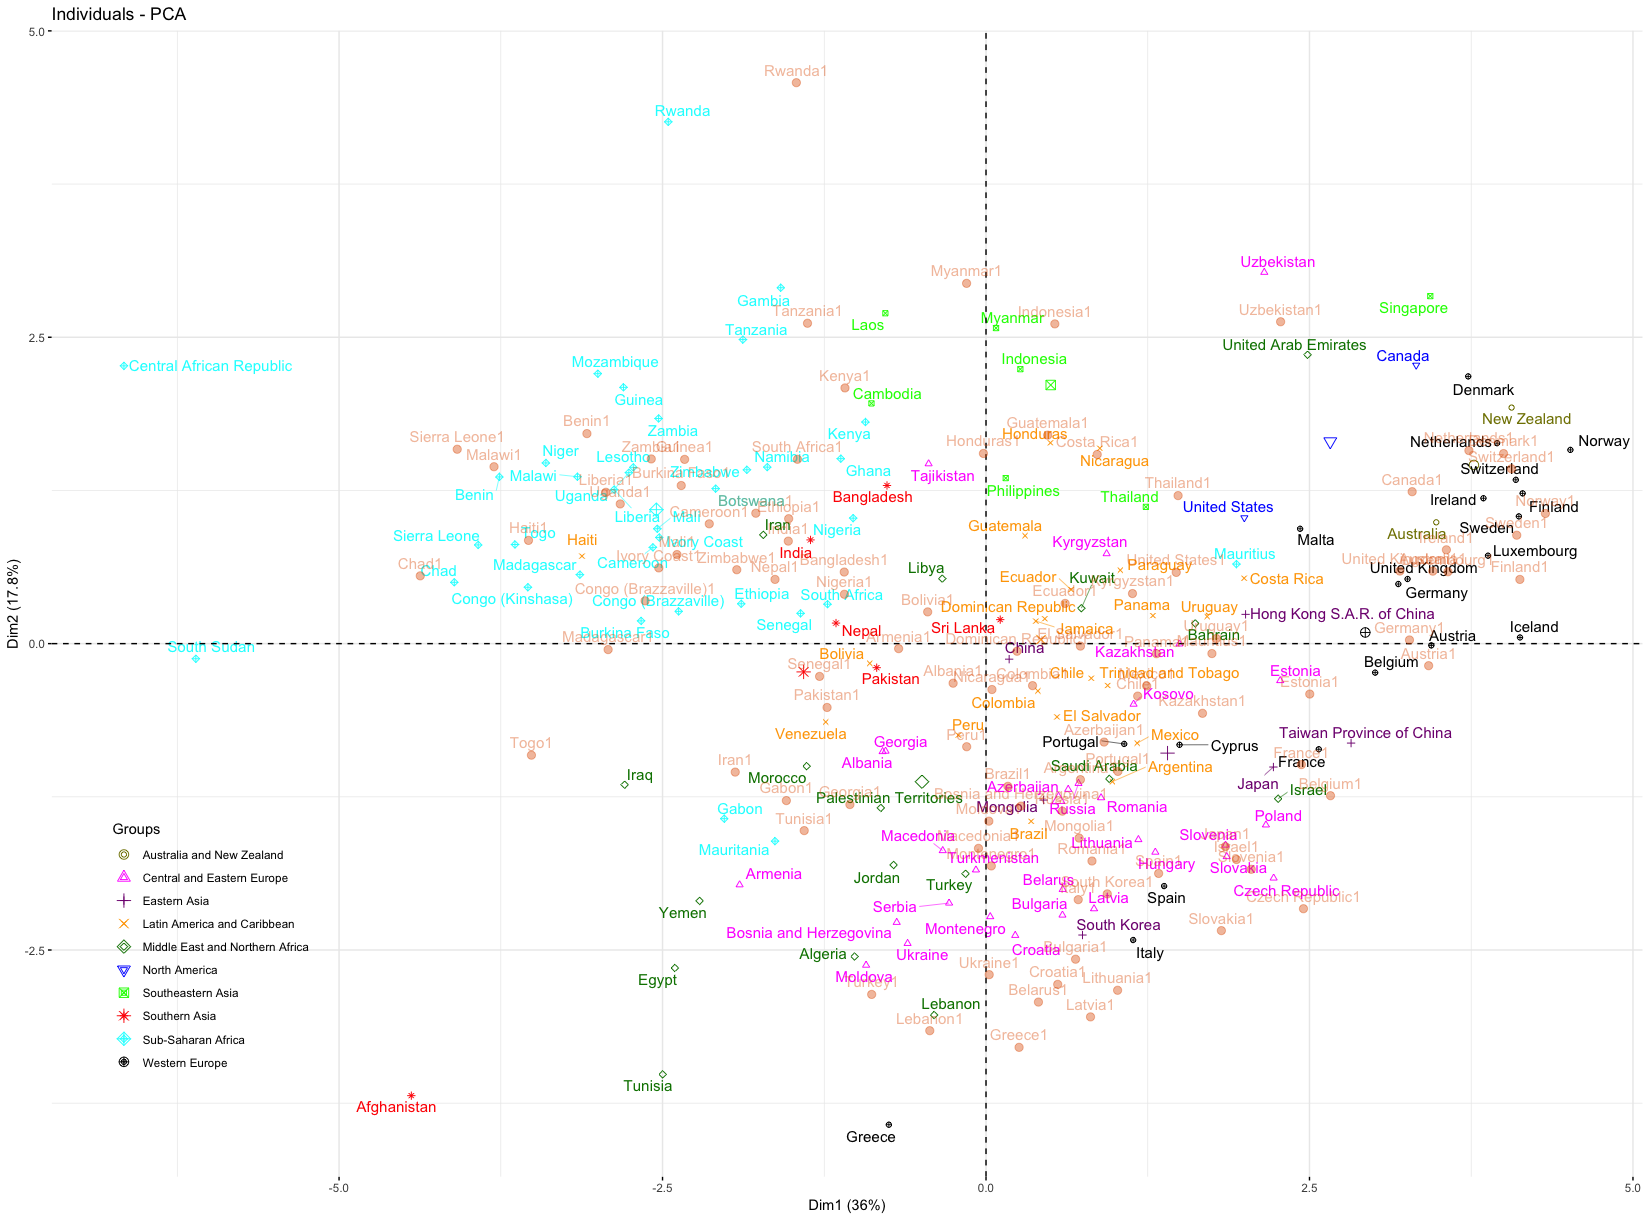
\includegraphics[width=1.1\textwidth]{figures/pca_individuals_suplementaries.png}
    \caption{Projected active and supplementary individuals, with active individuals color coded by region.\label{fig:pca-ind-sup}}
\end{figure}
\end{landscape}


\end{document}